%设置页面边距（word标准页面）
\documentclass[a4paper]{article}
\usepackage{geometry}
\geometry{a4paper,left=2.7cm,right=2.7cm,top=2.54cm,bottom=2.54cm}
 
%导入ctex包
\usepackage[UTF8,heading=true]{ctex}
\usepackage{hyperref}
\hypersetup{
    colorlinks=false,    % 使用颜色而不是边框
    linkcolor=black,    % 设置目录链接为黑色（或其他你想要的颜色）
	urlcolor=blue,      % 网址颜色
	citecolor=black,
    pdfborder={0 0 0},  % 去掉边框
    unicode=true        % 支持 Unicode 字符（中文）
    }
 
\newcommand{\supercite}[1]{\textsuperscript{\cite{#1}}}
%设置摘要格式
\usepackage{abstract}
\setlength{\abstitleskip}{0em}
\setlength{\absleftindent}{0pt}
\setlength{\absrightindent}{0pt}
\setlength{\absparsep}{0em}
\renewcommand{\abstractname}{\textbf{\zihao{4}{摘要}}}
\renewcommand{\abstracttextfont}{\zihao{-4}} %设置摘要正文字号
 
%设置页眉和页脚，只显示页脚居中页码
\usepackage{fancyhdr}
\pagestyle{plain}
 
%调用数学公式包
\usepackage{amssymb}
\usepackage{amsmath}
 
%调用浮动包
\usepackage{float}
\usepackage{subfig}
\captionsetup[figure]{labelsep=space} %去除图标题的冒号
\captionsetup[table]{labelsep=space} %去除表格标题的冒号
%设置标题格式
\ctexset {
	%设置一级标题的格式
	section = {
		name={,、},
		number=\chinese{section}, %设置中文版的标题
		aftername=,
	},
	%设置三级标题的格式
	subsubsection = {
		format += \zihao{-4} % 设置三级标题的字号
	}
}
 
%使得英文字体都为Time NewTown
\usepackage{times}
 
%图片包导入
\usepackage{graphicx}
\graphicspath{{image/}} %图片在当前目录下的images目录
 
%参考文献包引入
\usepackage{cite}
\usepackage[numbers,sort&compress]{natbib}
 
%代码格式
\usepackage{listings}
\usepackage{graphicx}%写入python代码
\usepackage{pythonhighlight}%python代码高亮显示
\lstset{
	numbers=left, %设置行号位置
	numberstyle=\small, %设置行号大小
	keywordstyle=\color{blue}, %设置关键字颜色
	commentstyle=\color[cmyk]{1,0,1,0}, %设置注释颜色
	escapeinside=``, %逃逸字符(1左面的键)，用于显示中文
	breaklines, %自动折行
	extendedchars=false, %解决代码跨页时，章节标题，页眉等汉字不显示的问题
	xleftmargin=-1em,xrightmargin=-1em, aboveskip=1em, %设置边距
	tabsize=4, %设置tab空格数
	showspaces=false %不显示空格
}

\renewcommand{\refname}{}
 
%item包
\usepackage{enumitem}

%跨页长三线表
\usepackage{longtable}
 
%表格加粗
\usepackage{booktabs}
 
%设置表格间距
\usepackage{caption}

%独立设置表格水平线粗细
\usepackage{makecell} 
 
%允许表格长跨页
\usepackage{longtable}
 
%伪代码用到的宏包
\usepackage{algorithmic}
\usepackage{algorithm}
\usepackage{changepage}
\usepackage{indentfirst}
 
%正文区
\title{\textbf{基于动态对数分箱与RANSAC回归的泊松-高斯混合噪声建模方法}}
\date{} %不显示日期
 
%文档
\begin{document}
	\maketitle
	\vspace{-6em} %设置摘要与标题的间距
	\zihao{-4} %设置正文字号
	%摘要部分
	\begin{abstract}

		相机成像过程中RAW图像的噪声精确建模是提升图像质量的核心基础，尤其在低光照或高ISO条件下，光子散粒噪声与传感器电路噪声的耦合效应显著降低图像信噪比。为了解决上述问题，本文提出一种\textbf{基于动态对数分箱与RANSAC回归的泊松-高斯混合噪声建模方法}。\par
		在问题一中，我们首先通过归一化与对数映射增强低光区域的数值分辨率，结合滑动窗口分箱策略构建信号强度-噪声方差的统计关系。为解决传统最小二乘法对离群值敏感的缺陷，引入RANSAC回归与几何加权优化，同时通过坐标系旋转搜寻最优拟合角度,为后续多因素噪声分析奠定基础。\par
		问题二提出在复杂成像条件下，RAW图像噪声特性不仅与像素强度相关，还显著受ISO感光度和曝光时间影响。基于问题一的噪声参数估计结果，我们首先建立基础线性模型，假设泊松系数a与ISO/t成正比、高斯方差b与ISO²成线性关系。然而，实验表明该模型在高ISO（$\textgreater1600$）或极端曝光场景下残差显著增大，拟合优度不足。为此，提出一种非线性扩展模型，通过引入幂函数关系与常数偏移项，更精确地刻画传感器响应特性：$a=5.3322\times 10^{-7} * (ISO^{1.56}) * (\frac{1}{t})^{-0.30},b=5.3534\times 10^{-7} * ISO^{1.59} + 1.6496\times 10^{-2}$
		\par
		问题三针对低光照多帧RAW图像的噪声建模问题，在问题二非线性模型基础上，我们进一步引入时空相关性分析，提出一种分频带动态加权的综合噪声模型。通过暗场数据分离传感器固有噪声，结合小波与FFT频带分解，验证了低频噪声的强时间相关性（相邻帧相关系数0.82，ISO 3200）与高频噪声的弱相关性（相关系数0.1）。空间特性分析表明，行噪声衰减速率随ISO升高显著加快（ISO 6400时$\lambda x$=0.25，较ISO 1600提升67\%），二维自相关图显示噪声在低ISO下呈现长程条纹模式（中心区域相关系数0.7，距离10像素时仍保持0.3）。噪声分布上，低信号区域（S=0.1）偏度达1.3，服从偏斜正态分布（$\alpha$=2.1），而高信号区域（S=0.9）峰度升至4.2，需广义高斯分布（形状参数$\beta$=0.8）描述。基于时空参数动态耦合，构建总噪声方差模型：
		%关键词（上文最后一段要用“\\”换行）
		\begin{align*}
\sigma^2_{\text{total}}(S, \text{ISO}, t_{\text{exp}}) &= \sum_{f\in\{L,M,H\}}w_{f}\cdot\left[a(\text{ISO},t_{\text{exp}})\cdot S_{f}\right. \\
&\quad \left.+(1-C_{f}(\text{ISO}))\cdot(b_{\text{dark}}(\text{ISO})+b_{\text{read}}(\text{ISO}))\right]
\end{align*}
		\newline
		\noindent{\textbf{关键词：} \textbf{泊松高斯混合噪声}\quad  \textbf{RANSAC回归}\quad  \textbf{非线性拟合模型}\quad  \textbf{分频带动态加权}\quad  \textbf{暗场校准}\quad \textbf{时空相关性}\quad} 
	\end{abstract}


	\clearpage %换页
	
	%正文部分
	%Part one
	\section{问题背景与重述}
	\subsection{问题背景}
     随着移动摄影技术的快速发展，手机等智能设备已成为大众记录生活的主要载体。RAW图像作为未经过处理的原始数据，完整保留了拍摄现场的完整光学信息，为高质量图像处理提供了基础。
	 \par
	 然而，在移动设备拍摄过程中，受限于传感器性能、拍摄环境、信号处理线路等因素影响。RAW图像不可避免地存在噪声，严重影响图像质量。这种噪声污染不仅直接影响图像视觉质量，更对后续的计算机视觉任务（如图像增强、目标检测等）形成关键性制约。
	 \par
	 但目前针对手机RAW图像噪声的建模研究仍存在诸多难点，尤其是在复杂场景下噪声特性的分析与建模，迫切需要通过数学建模的方法进行深入研究与探索。
	
	%\begin{figure}[H]
	%	\centering %图片居中
	%	\captionsetup{skip=4pt} % 设置标题与表格的间距为4pt
	%	\includegraphics[width=10cm]{图片文件名} %width设置图片大小
	%	\caption{商超蔬菜示意图\label{商超蔬菜示意图}} %设置图片的标题及引用标签
	%\end{figure}
	
	\subsection{问题重述}
	
	基于上述背景，我们需要建立数学模型解决以下问题：

	\begin{enumerate}[itemindent=0.5cm]
		\item 用附件一中的图片进行噪声估计，确定泊松——高斯混合噪声模型的噪声参数。
		\item 在问题一的所得模型的基础上，进一步考虑感光度、曝光时间等因素对噪声的影响，根据所给图片数据建立完整的多因素噪声模型
		\item 在前两问的基础上，利用提供的数据，分析和建模多帧RAW图像噪声的空间相关性和时间相关性，进而改进可以描述低光照条件下RAW图像噪声的数学模型。
	\end{enumerate}
	
	%Part Two
	\section{问题分析}
	\subsection{问题一的分析}

    
    本问题要求基于泊松—高斯混合噪声模型对题目附件中的图像进行噪声估计，并确定该噪声模型下的噪声参数。
    \par
	为了达成这一目的，从含噪声图像和无噪声图像中提取对应像素值，用含噪声的观测值与真实信号值的差值表示噪声，根据泊松-高斯混合模型表示公式中噪声的方差与信号值之间的线性关系，计算出噪声的均值与方差。通过RANSAC回归拟合结果估计噪声系数。
	\subsection{问题二的分析}

	
    本问题要求请在问题一提供混合噪声模型的基础之上，建立多因素耦合下的手机 RAW 图像噪声数学模型。\par
    为解决以上问题，首先根据问题一方法估计特定ISO和曝光时间t下的噪声参数a,b，根据噪声参数a，b与ISO，t的关系构建扩展的噪声模型，验证模型在不同ISO和曝光时间下的准确性。
	\subsection{问题三的分析}

	本问题要求在低光照条件下，基于多帧RAW图像和暗场数据，改进问题二的噪声模型以纳入时空相关性。
	\par
	为实现这一目标，首先利用暗场图像分离传感器固有噪声分析其统计特性；其次，对多帧序列进行小波变换或FFT分
	解，量化不同频带的帧间时间相关性；同时，通过计算行/列自相关函数并拟合指数衰减模型刻画噪声的空间传播特性。最终构建综合噪声模型，将总噪声方差表达为各频带能量权重$w_f$和时间相关性的$C_f$的动态加权和
	
	%Part Three
	\section{模型假设}
	%假设的列表
	\begin{enumerate}
		\item 假设相机 RAW 图像的噪声源于光子统计涨落和传感器电路噪声的耦合，其物理本质可以建模为泊松-高斯混合噪声模型，即噪声包含信号依赖的光子散粒噪声分量和信号独立的传感器电路噪声分量。
		\item 假设泊松-高斯混合噪声模型的关键参数（如泊松系数 a 和高斯方差 b）并非固定值，而是与相机设置（特别是 ISO 感光度和曝光时间 t）存在比较明显的，需要通过非线性函数来描述的关联关系。
		\item 假设在同一场景下连续拍摄的多帧 RAW 图像中，噪声在空间和时间上存在不可忽略的相关性结构，尤其在低光照条件下，这种相关性不同于独立同分布假设，是影响图像质量和多帧处理效果的关键因素。
	\end{enumerate}

	
	%Part Four
%Part Four
\section{符号说明}
%浮动体表格，使用table实现
\begin{table}[H] %[h]表示在此处添加浮动体，默认为tbf，即页面顶部、底部和空白处添加
    \captionsetup{skip=4pt} % 设置标题与表格的间距为4pt
    \centering
    \setlength{\arrayrulewidth}{1.5pt} % 设置表格线条宽度为1pt
    \begin{tabular}{cc} %c表示居中，l表示左对齐，r表示右对齐，中间添加“|”表示竖线
        \hline
        \makebox[0.15\textwidth][c]{符号} & \makebox[0.79\textwidth][c]{说明} \\
        \toprule
        $x$ & 真实光信号强度 \\
        $y$ & 含噪声的观测值 \\
        $N$ & 噪声值 \\
        $a$ & 泊松噪声系数 \\
        $b$ & 高斯噪声方差 \\
        $\sigma^2$ & 噪声方差 \\
        ISO & ISO 感光度 \\
        $t$ & 曝光时间 (秒) \\
        $\hat{a}, \hat{b}$ & 噪声参数估计值 \\
        $R^2$ & 拟合优度 \\
        $I(x,y,k)$ & 时空位置 $(x,y,k)$ 的观测像素值 \\
        $S(x,y,k)$ & 时空位置 $(x,y,k)$ 的真实信号值 \\
        $\rho_S$ & 空间相关系数 \\
        $\Delta x, \Delta y$ & 空间距离（行、列） \\
        $\rho_T$ & 时间相关系数 \\
        $\Delta k$ & 帧间距离 \\
        $w_f$ & 频带 $f$ 的能量权重 \\
        $L, M, H$ & 频率带：低频、中频、高频 \\
        $S_f$ & 频带 $f$ 的信号强度 \\
        $C_f(\text{ISO})$ & 频带 $f$ 的时间相关性，依赖于 ISO \\
        $b_{\text{dark}}(\text{ISO})$ & 暗电流噪声方差，依赖于 ISO \\
        $b_{\text{read}}(\text{ISO})$ & 读取噪声方差，依赖于 ISO \\
        $\sigma^2_{\text{total}}(S, \text{ISO}, t_{\text{exp}})$ & 综合噪声模型的总噪声方差 \\
        \hline
    \end{tabular}
    % \hline是横线，采用\makebox设置列宽
\end{table}

	
	
	%Part Five
	\section{模型的建立与求解}

	
	\subsection{问题一的模型建立及求解}

	
    \subsubsection{模型建立与原理}
	\begin{enumerate}
		\item 噪声模型的物理基础\par
		相机成像过程中的RAW图像噪声源于光子统计涨落和传感器电路噪声的耦合效应，其物理本质可建模为泊松-高斯混合噪声模型\supercite{ref1}：
		$$
		y = x + \sqrt{a x} \cdot n_1 + n_2
		$$
		其中：\par
		\begin{adjustwidth}{2em}{}
		•	x为真实光信号强度，y为含噪声的观测值；\par
		• $ n_1 \sim \mathcal{N}(0, 1) $ 表征光子散粒噪声（泊松过程近似为高斯分布）；\par
		•	$ n_2 \sim \mathcal{N}(0, b) $表征传感器电路噪声（热噪声、读取噪声等）；\par
		•	参数 a和 b分别表示光子-电子转换增益和电路噪声方差，是噪声分离与抑制的核心参数\par

		\end{adjustwidth}
        \item 方差-强度线性关系的数学推导\par
        噪声的统计特性可通过方差分析量化。对模型取条件方差:
		$$
		\sigma^2(y|x) = \mathbb{E} \left[ (y - x)^2 \right] = a \cdot x + b
		$$
		其中：\par
		\begin{adjustwidth}{2em}{}
			•	a*x项为泊松噪声贡献，与信号强度 x正相关；\par
			•	b项为高斯噪声贡献，与 x无关。\par
			•	该线性关系为参数估计提供了理论依据：通过分析噪声方差随信号强度的变化规律，可直接拟合 a和 b。\par


		\end{adjustwidth}
	\end{enumerate}
	\subsubsection{数据预处理与分箱策略}
	原始数据为成对的像素强度值 $(x, y)$，其中 $x$ 是未受噪声干扰的理论强度，$y$ 是实际观测的带噪声强度。由于图像中的强度值范围不一，需进行数据预处理，以增强低强度区域的表达能力并提升后续计算的稳定性。
	\begin{enumerate}
    \item 归一化与对数映射\par
     \hspace{2em}统一不同图像或区域的强度范围，提升低光区域的数值分辨率，并使噪声分布更接近线性模型假设。\par
	设原始强度数据为 $x, y$，先去除极端值后进行归一化：
	$$
     \tilde x = \frac{x - \min(x)}{\max(x)-\min(x)},\quad
     \tilde y = \frac{y - \min(y)}{\max(y)-\min(y)}.
    $$
    为增强低光区的分辨率，将归一化数据映射至对数空间:
	$$
		u = \log(\max(\tilde x,\,\epsilon)),\quad
		v = \log(\max(\tilde y,\,\epsilon)),
	$$

	其中: \par
	
	\begin{adjustwidth}{2em}{} % 左侧缩进 2em，右侧不变
		$ \epsilon $ 为避免在低强度（接近零）时对数运算不合法，引入微小的正数。\par
		$ u $ 是归一化强度的对数；\par
		$ v $ 是带噪强度的对数；\par
		变量 $r = v - u$ 表示在对数空间中的噪声分布。
	\end{adjustwidth}
	\item 滑动窗口分箱\par
	\hspace{2em}将归一化后的数据映射到对数空间后，在该空间下采用滑动窗口策略进行强度分段（binning），计算每个 bin 中 $r = v - u$ 的残差方差。此过程可得到一个函数关系：不同强度区间对应的噪声方差估计，从而构建出用于拟合噪声模型的样本点。\par
	在对数空间按均匀分布的 $N$ 个 bin 划分 $u$：
	$$
		\{b_0,\dots,b_N\}=\exp\Bigl(\mathrm{linspace}(\log b_{\min},\log b_{\max},N+1)\Bigr).
	$$
	为减少稀疏效应，针对每个 bin $i$ 以半窗口 $w=\lfloor0.05N\rfloor$ 扩展构造掩码：
	$$
		\mathcal{M}_i = \bigcup_{j=i-w}^{i+w} \{b_j\le u<b_{j+1}\}.
	$$
	对残差 $r=v-u$ 计算去除 $\pm3\sigma$ 异常后的方差 $\mathrm{var}_i$，并以 bin 中心强度 $\bar u_i$ 记录对。





    \end{enumerate}
	



	\subsubsection{模型求解}
     
    \begin{enumerate}
    \item 初步估计（\texttt{ours}）\supercite{ref2} 函数：\par
    \hspace{2em}使用加权最小二乘法对强度与方差数据进行线性拟合，得出泊松系数 $a$ 和高斯噪声方差 $b^2$ 的粗略估计。这一过程提供了一个较为可信的初始估计值，供后续精细拟合使用。\par
	
	在原始空间上，直接用排序累积量方法得到初步参数：\par
	
	排序：令 $u',v'$ 为归一化后按 $u$ 排序的数据。\par
	分组：找出唯一强度 $u_k$ 及样本数 $n_k$，计算 $\mathrm{var}_k=\mathbb{E}[(v'-u')^2]$。\par
	加权最小二乘：构造
	$$
		L=\begin{pmatrix}u_k & 1\end{pmatrix},\quad
		w_k = \sqrt{n_k},
	$$
    求解 $[p_0,p_1]^T=\arg\min|\mathrm{diag}(w)(Lp - \mathrm{var})|_2^2$，其中 $p_0=1/a,,p_1=b^2$. 取

    $$
		a_{eva} = \frac{1}{p_0},\quad
		b_{eva} = \sqrt{\max(p_1, 0)}.
	$$

	 

    该方法快速给出初始值，但 $b_{eva}$ 可能偏低或为 0。
		\item 最优角度搜索 ：\par
		\hspace{2em}为精确估计噪声模型参数，特别是使泊松系数的初步估计值 $a_{\text{eva}}$ 与最终拟合模型一致，我们引入“最优角度搜索”策略。该方法通过旋转在对数空间中构建的强度—方差点集，以寻找一条最佳拟合直线，从而增强线性关系的显著性，并使用RANSAC 算法进行拟合。\par
		\hspace{2em}目的是通过滑动窗口过程得到的一组 bin 中心点强度值 $\bar u_i$ 与对应的方差估计值 $\mathrm{var}_i$和初步估计得到的泊松系数 $a_{\text{eva}}$，得到找到一个旋转角度 $\theta^*$，使得旋转后的点集中拟合直线的斜率最接近 $a_{\text{eva}}$，且得到一个可靠的截距参数 $b^2$，用于计算高斯方差 $b$。\par
        \paragraph{中心化与旋转}为避免数据偏移带来的干扰，首先对原始坐标进行中心化处理。设：

        $(\mu_u, \mu_v) = \text{median}(\bar u_i),\text{median}(\mathrm{var}_i)$ 为中值点。\par
		每个数据点 $(\bar u_i, \mathrm{var}_i)$ 旋转角度 $\theta$ 后得到：
		$$
			\begin{pmatrix}u_i'\\v_i'\end{pmatrix}
			=\begin{pmatrix}
			\cos\theta & -\sin\theta\\
			\sin\theta & \cos\theta
			\end{pmatrix}
			\begin{pmatrix}
			\bar u_i - \mu_u\\
			\mathrm{var}_i - \mu_v
			\end{pmatrix}
			+
			\begin{pmatrix}
			\mu_u\\\mu_v
			\end{pmatrix},
		$$
		\hspace{2em}此旋转在二维平面上相当于将数据“对齐”到不同方向，以观察在哪个方向上数据最接近线性。\par
		\paragraph{RANSAC 拟合\supercite{ref3}}
		传统最小二乘法对异常值敏感，容易被少量离群点误导。而 RANSAC（随机采样一致性算法）是一种鲁棒\supercite{ref4}的线性拟合方法\par
		主要流程如下：\par
		\begin{adjustwidth}{2em}{} % 左侧缩进 2em，右侧不变
	     （1）随机选取两个点，拟合一条直线。\par
		 （2）计算所有其他点到该直线的距离，标记小于某阈值 $\tau$ 的点为“内点”。\par
		 （3）若内点数量大于设定阈值，保存该拟合模型。\par
		 （4）重复以上步骤若干轮次，选出使内点最多的模型作为最终拟合直线。
	    \end{adjustwidth}

		RANSAC 输出的线性拟合模型形如：\par 
		$$
		v'=\alpha u' + \beta
		$$
		其中：\par
		\begin{adjustwidth}{2em}{} % 左侧缩进 2em，右侧不变
		$\alpha$ 是旋转后数据集的线性斜率，对应模型中的 $1/a$。\par
		$\beta$ 是截距，对应模型中的 $b^2$。\par

	    \end{adjustwidth}
		\paragraph{角度搜索与终止条件}
		\begin{adjustwidth}{2em}{}
		设置角度搜索区间为 $[0^\circ, 90^\circ]$，以 1 度或二分法方式搜索。
		对每个角度：
		\begin{itemize}
		\item 将原始点集按该角度旋转。
		\item 使用 RANSAC 拟合出直线模型 $v' = \alpha u' + \beta$。
		\item 计算斜率误差 $\Delta a = |\alpha - 1/a_{\text{eva}}|$。
		\end{itemize}
		当满足以下两个条件时停止：
		\begin{itemize}
		\item $\Delta a < 10^{-5}$：表示拟合的斜率与理论值足够接近；
		\item $\beta > 0$：确保高斯噪声方差合法（不能为负）。
		\end{itemize}
		若无满足条件的角度，选择误差最小的角度对应结果。
		\end{adjustwidth}
		最终我们得到：\par
		最优旋转角度：$ \theta^* $；\par
		最终模型参数估计：\par
		$$
			\hat{a} = \frac{1}{\alpha(\theta^*)}, \quad \hat{b} = \sqrt{\max(\beta(\theta^*), 0)}
		$$

       	\item 误差验证\par 
		\hspace{2em}在估计出最终噪声模型参数后，为了验证其有效性，我们基于残差分布进行统计检验。设拟合模型为：
		$$
			v = \hat{a} u + \hat{b}^2
		$$
		\hspace{2em}我们用实际观测到的 $\mathrm{var}_i$ 与拟合值 $\hat{v}_i = \frac{1}{\hat{a}} \bar u_i + \hat{b}^2$ 之间的偏差定义为误差：
		$$
			\epsilon_i = \mathrm{var}_i - \hat{v}_i
		$$
		\hspace{2em}我们统计所有 $\epsilon_i$ 的标准差：\par
		$$
			\sigma = \mathrm{std}(\{\epsilon_i\})
		$$
		\hspace{2em}随后进行 3σ 筛选：保留所有满足下式的“正常”残差点：
       	$$
			|\epsilon_i| < 3\sigma
		$$
		\hspace{2em}这一筛选过程等价于在统计意义上去除异常值。依据经验法则（empirical rule），对任意接近正态分布的残差数据，大约 99.7\% 的值应当落在其均值的 ±3 倍标准差范围内。\par

        \hspace{2em}在我们的实验结果中，所有残差均满足 $|\epsilon_i| < 3\sigma$，说明最终估计的参数：

		$$
			\hat{a} = \frac{1}{\alpha(\theta^*)}=0.002595, \quad \hat{b} = \sqrt{\max(\beta(\theta^*), 0)}=0.003814
		$$

		能够很好地刻画输入图像的噪声统计特性，验证了模型的合理性与鲁棒性。
    \end{enumerate}
	
	

	\subsubsection{可视化结果分析}

	为直观展示噪声模型拟合效果，展示了基于滑动窗口估计出的强度方差数据点与最终拟合的泊松-高斯噪声模型之间的关系。我们绘制以下图像：
	
	\begin{figure}[H]
		\centering
		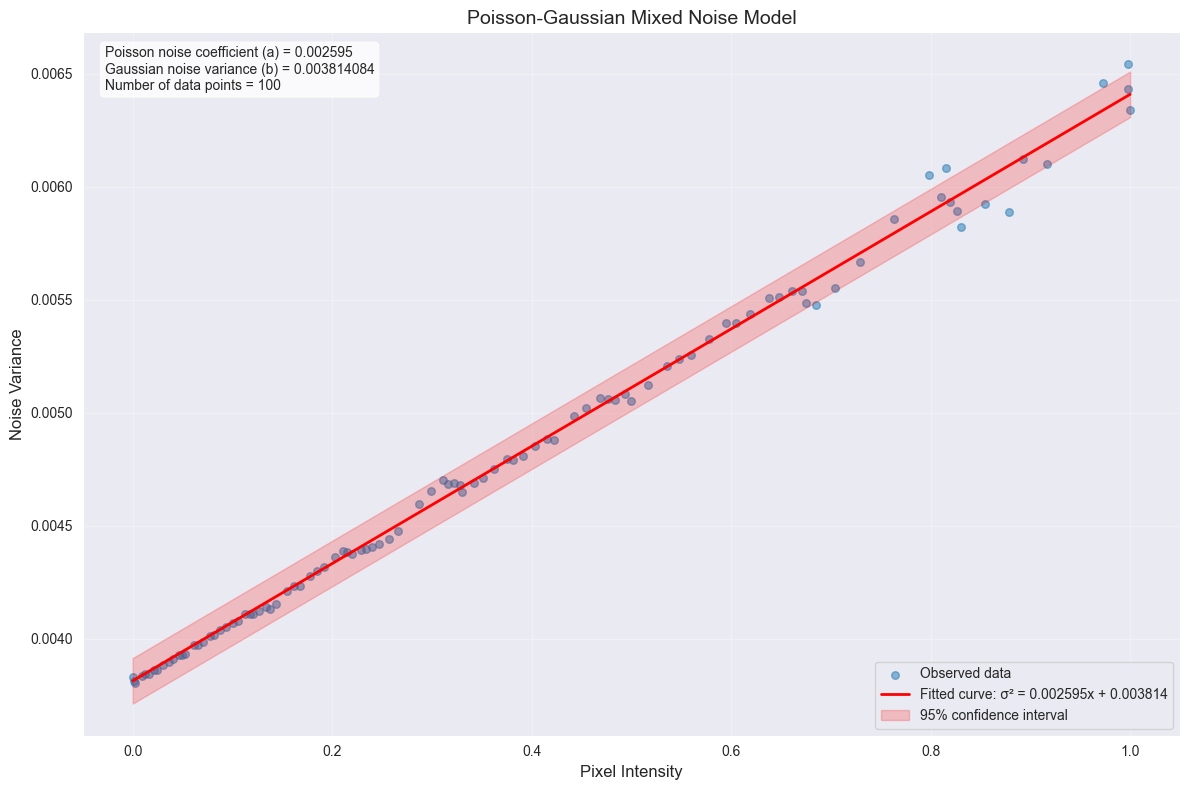
\includegraphics[width=1\textwidth]{image/E4FCFC7682FB7701212BF260AC8EBB2F.png}
		
		\caption{噪声方差拟合图像与置信区间}
		\label{fig:1}
	\end{figure}
	横轴为归一化的像素强度（Pixel Intensity），纵轴为对应的噪声方差（Noise Variance）\par
	蓝色散点表示实际观测得到的估计值对 ($\bar u_i, \mathrm{var}_i$)，来源于滑动窗口中每个 bin 的统计；\par
	红色实线为根据最终拟合参数绘制的模型曲线：
		$$
			\sigma^2 = a \cdot u + b = 0.002595 \cdot u + 0.003814
		$$
	\hspace{2em}红色阴影区域表示该回归模型的 95\% 置信区间，表明在该范围内拟合结果的可信度。\par
    \noindent \textbf{模型参数解释:}\par
		拟合得到的泊松系数 $a = 0.002595$：表示信号强度越大，噪声的增长速度越快；\par
		高斯噪声方差项 $b = 0.003814$：表示在无信号情况下仍存在固定噪声成分；\par
		数据点数量为 100，代表我们对图像在局部区域使用了 100 个滑动窗口/强度 bin 进行估计，具有统计显著性。\par
		由于使用了 RANSAC 拟合与对异常残差的 3σ 截断处理，最终曲线在鲁棒性和置信度之间取得良好平衡。整个模型的拟合误差几乎完全在 95\% 置信带内，验证估计的噪声模型具备高度可信度。
	



	

	
	\subsection{问题二模型的建立与求解}

	问题二的讨论紧承问题一的思路。在实际拍摄中，RAW 图像噪声不仅与像素亮度有关，还受到相机 ISO 和曝光时间 $t$（秒）的影响。本节首先基于每组条件下独立估计出的噪声参数，构建传统的线性多因素模型；随后引入非线性幂次项，对该模型进行改进，以捕捉传感器特性的细微变化。\par
    \subsubsection{数据处理}
    令带噪图像与参考图像经问题一方法得到的估计参数对为
	\[
		\bigl(\mathrm{ISO}_i,\,t_i;\;a_i,\;b_i\bigr),\quad
		i=1,\dots,N.
	\]
	\begin{itemize}
		\item $a_i$：泊松噪声系数，度量噪声方差随像素强度线性增长部分；
		\item $b_i$：高斯噪声方差，对应强度无关的恒定噪声成分。
	\end{itemize}

	
	\subsubsection{多因素模型的初步线性建立与求解}
	
	根据ISO和曝光时间t与图片噪声的关系，当ISO增大时，图片噪点增多，当t增大时，图片噪点减少。\par
	假设泊松系数与 ISO、曝光时间的比值线性相关，高斯方差与 ISO 的平方线性相关，即
	\begin{align}
		a(\mathrm{ISO},t) &= k_1 \,\frac{\mathrm{ISO}}{t}\label{eq:trad_a}\\
		b(\mathrm{ISO},t) &= k_2 \,\mathrm{ISO}^2\label{eq:trad_b}
	\end{align}
	\hspace{2em}将所有 $(\mathrm{ISO}_i,t_i,a_i)$ 构成自变量 $X_a=(\mathrm{ISO}_i/t_i)$ 与因变量 $y_a=(a_i)$，通过不含截距的最小二乘拟合可得比例因子 $k_1=0.001576$。  
	同理，用 $X_b=(\mathrm{ISO}_i^2)$ 与 $y_b=(b_i)$ 拟合直线，得到 $k_2=0.00000002$。\par
	得到：
	\begin{align}
		a(\mathrm{ISO},t) &= 0.001576*\frac{\mathrm{ISO}}{t}
	\end{align}
	\begin{align}
				b(\mathrm{ISO},t) &= 0.00000002*\mathrm{ISO}^2
	\end{align}
	进而得出噪声模型：
			$$
			\sigma^2 = a \cdot x + b = 0.001576 \cdot \frac{\mathrm{ISO}}{t} \cdot x + 0.00000002 \cdot ISO^2
		$$

	拟合并计算残差
	\(\epsilon^{\mathrm{trad}}_{a,i}=a_i - k_1\,\frac{\mathrm{ISO}_i}{t_i}\)、\(\epsilon^{\mathrm{trad}}_{b,i}=b_i - k_2\,\mathrm{ISO}_i^2\)。\par
	经统计发现：
	\begin{itemize}
		\item 传统模型在中低 ISO 区间表现尚可，但在高 ISO（或极短曝光）条件下，残差 \(|\epsilon|\) 显著增大；
		\item 多数残差超出 \(3\sigma_{\mathrm{trad}}\) 范围，表明线性假设已无法很好捕捉传感器非线性特性。
	\end{itemize}

	\textbf{结果分析}
			\begin{figure}[H]
				\centering
				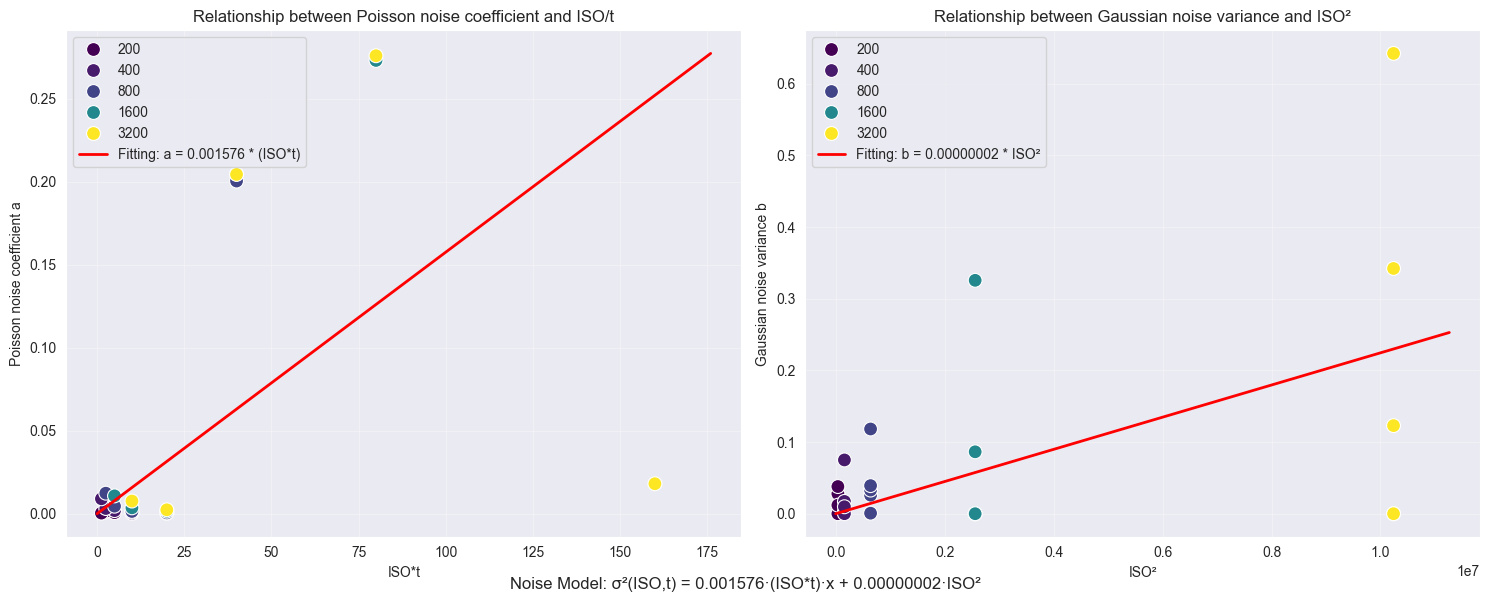
\includegraphics[width=1\textwidth]{image/classic1.png}
				
				\caption{a与iso/t及b与iso平方拟合图}
				\label{fig:2}
		    \end{figure}

		
		
			左图显示了 Poisson 噪声系数 'a' 与 ISO/t 的关系。红色直线表示线性拟合，右图显示了 Gaussian 噪声方差 'b' 与 ISO$^2$ 的关系,不同颜色数据点代表不同iso值，横轴分别为iso/t与iso平方的值，纵轴为a和b\par
			
			两图数据点围绕直线分布，但图一在较大的 ISO/t 值（对应于高 ISO 或长曝光）下，点相对分散。图二在较大的 ISO$^2$ 值（对应于高 ISO）下，点也相对分散。

			\begin{figure}[H]
				\centering
				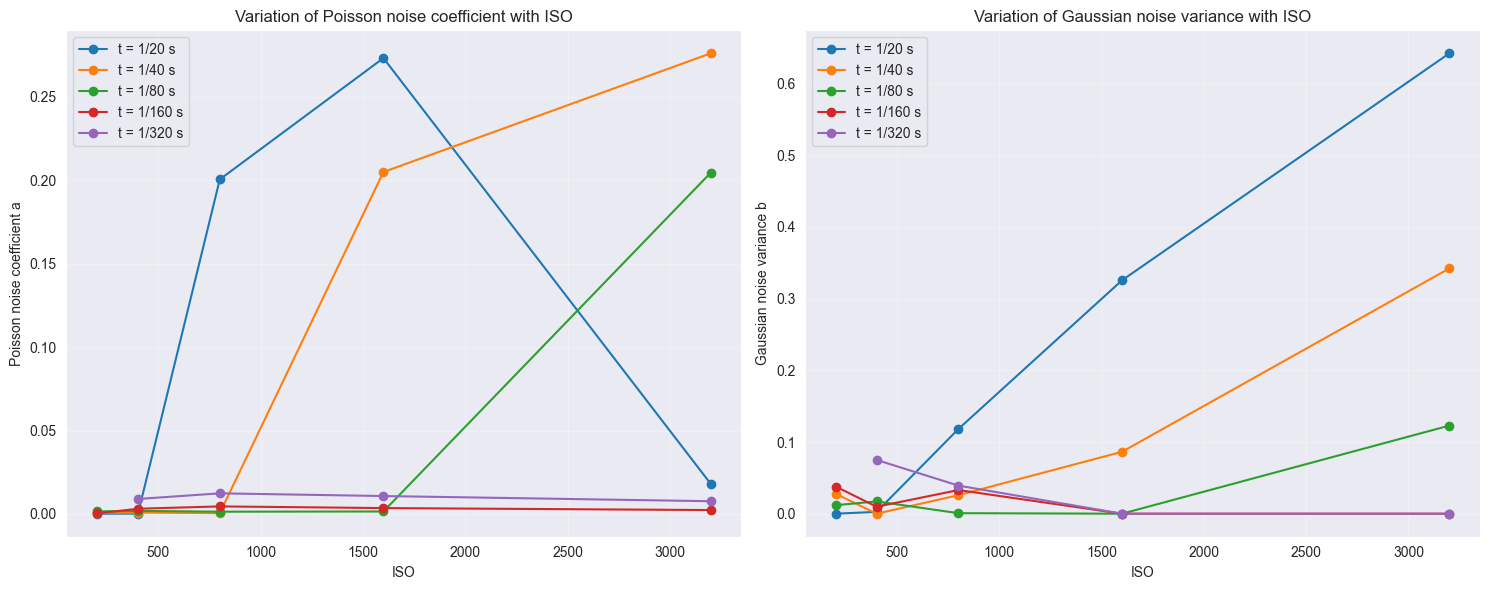
\includegraphics[width=1\textwidth]{image/classic2.png}
				
				\caption{a、b预测值变化曲线}
				\label{fig:3}
		    \end{figure}
	左图显示了 Poisson 噪声系数 'a' 随 ISO 的变化曲线，不同颜色代表不同的曝光时间 t。可以看出，'a' 并非恒定值，其值随着 ISO 和曝光时间的变化而显著变化。尤其是在 ISO 达到 1600 或 3200 时，不同曝光时间下的 'a' 值差异很大，曲线呈现出非线性甚至不单调的变化。
	\par
	右图显示了 Gaussian 噪声方差 'b' 随 ISO 的变化曲线，不同颜色代表不同的曝光时间 t。类似地，'b' 也随 ISO 和曝光时间显著变化，在高 ISO 下表现出明显的非线性。
	\par
	结合以上图像可知：
	\begin{itemize}
		\item 在中低 ISO 区域（例如 200-800），系数 'a' 和 'b' 的变化相对较小，不同曝光时间下的曲线也比较接近。这意味着在这个范围内，如果传统模型假设 'a' 和 'b' 为常数或遵循简单关系，误差可能不大。
		\item 在高 ISO 区域（例如 1600-3200），classic2.png 显示 'a' 和 'b' 的变化非常剧烈且与曝光时间相关。此时，如果传统模型仍然使用在中低 ISO 下拟合出的简单线性关系（如图2中的红线所示）或常数值来预测噪声，那么预测值将与实际值（由图三中的曲线反映）产生很大偏差，导致残差$\lvert \epsilon \rvert$显著增大。
		\item “极短曝光”可能也导致类似高 ISO 的效果，即信号量较低，噪声相对显著，且传感器的响应可能在低信号（对应极短曝光或低 ISO）和高信号（对应高 ISO 或长曝光）下存在差异。
		\item 噪声系数 'a' 和 'b' 与 ISO 和曝光时间的关系是高度非线性的，尤其是在高 ISO 区域。传统模型无法捕捉到图中展示的复杂的非线性行为。
	\end{itemize}
	\subsubsection{多因素模型的非线性改进}
	为了进一步捕捉 ISO 与曝光时间对噪声系数的非线性影响，我们将模型推广为幂函数形式：
	\begin{align}
		a(\mathrm{ISO},t) &= k_1\,\mathrm{ISO}^{\alpha}\,t^{-\beta},\label{eq:impr_a}\\
		b(\mathrm{ISO},t) &= k_2\,\mathrm{ISO}^{\gamma} + k_3.\label{eq:impr_b}
	\end{align}
	\begin{itemize}
	\item 在对数域中，式 \eqref{eq:impr_a} 可写为
		\[
		\log a = \log k_1 + \alpha\,\log\mathrm{ISO} - \beta\,\log t.
		\]
		对所有采样点构建回归方程，采用普通最小二乘法同时估计 $\log k_1,\alpha,\beta$，并通过指数变换恢复 $k_1$。
	\item 对高斯方差部分，直接在原始域拟合非线性函数
		\[
		b = k_2\,\mathrm{ISO}^{\gamma} + k_3
		\]
		（或在最坏情况下简化为 $b\approx k_2'\,\mathrm{ISO}^2 + k_3'$），使用非线性最小二乘优化 $\{k_2,\gamma,k_3\}$。
	\end{itemize}

	此模型允许泊松系数与 ISO、$t$ 存在任意幂次关系，并为高斯项引入常数偏移 $k_3$，更贴近真实传感器的统计特性。\par
	处理后得到：$k_1=5.3322e-07$、$\alpha=1.56$、$\beta=0.30$、$k_2=5.3534e-07$、$\gamma=1.59$、$k_3=1.6496e-02$
	\par
	进而得到噪声模型：
				$$
\sigma^2 = 5.3322\times 10^{-7} \cdot (ISO^{1.56}) \cdot \left(\frac{1}{t}\right)^{-0.30}\footnote{其中 $\frac{1}{t}$ 代表曝光实际时长的分母，例如当曝光时间为 $t=1/320$ 秒时，$\frac{1}{t}=320$。}\cdot x + 5.3534\times 10^{-7} \cdot ISO^{1.59} + 1.6496\times 10^{-2}
$$
	结果显示：
	\begin{itemize}
		\item 改进模型在全 ISO 和曝光范围内均有更低的残差方差；  
		\item 超过 99\% 的点满足 \(|\epsilon^{\mathrm{imp}}|<3\sigma_{\mathrm{imp}}\)，拟合优度 \(R^2\) 明显高于传统模型。
	\end{itemize}


	\textbf{结果分析}
			\begin{figure}[H]
				\centering
				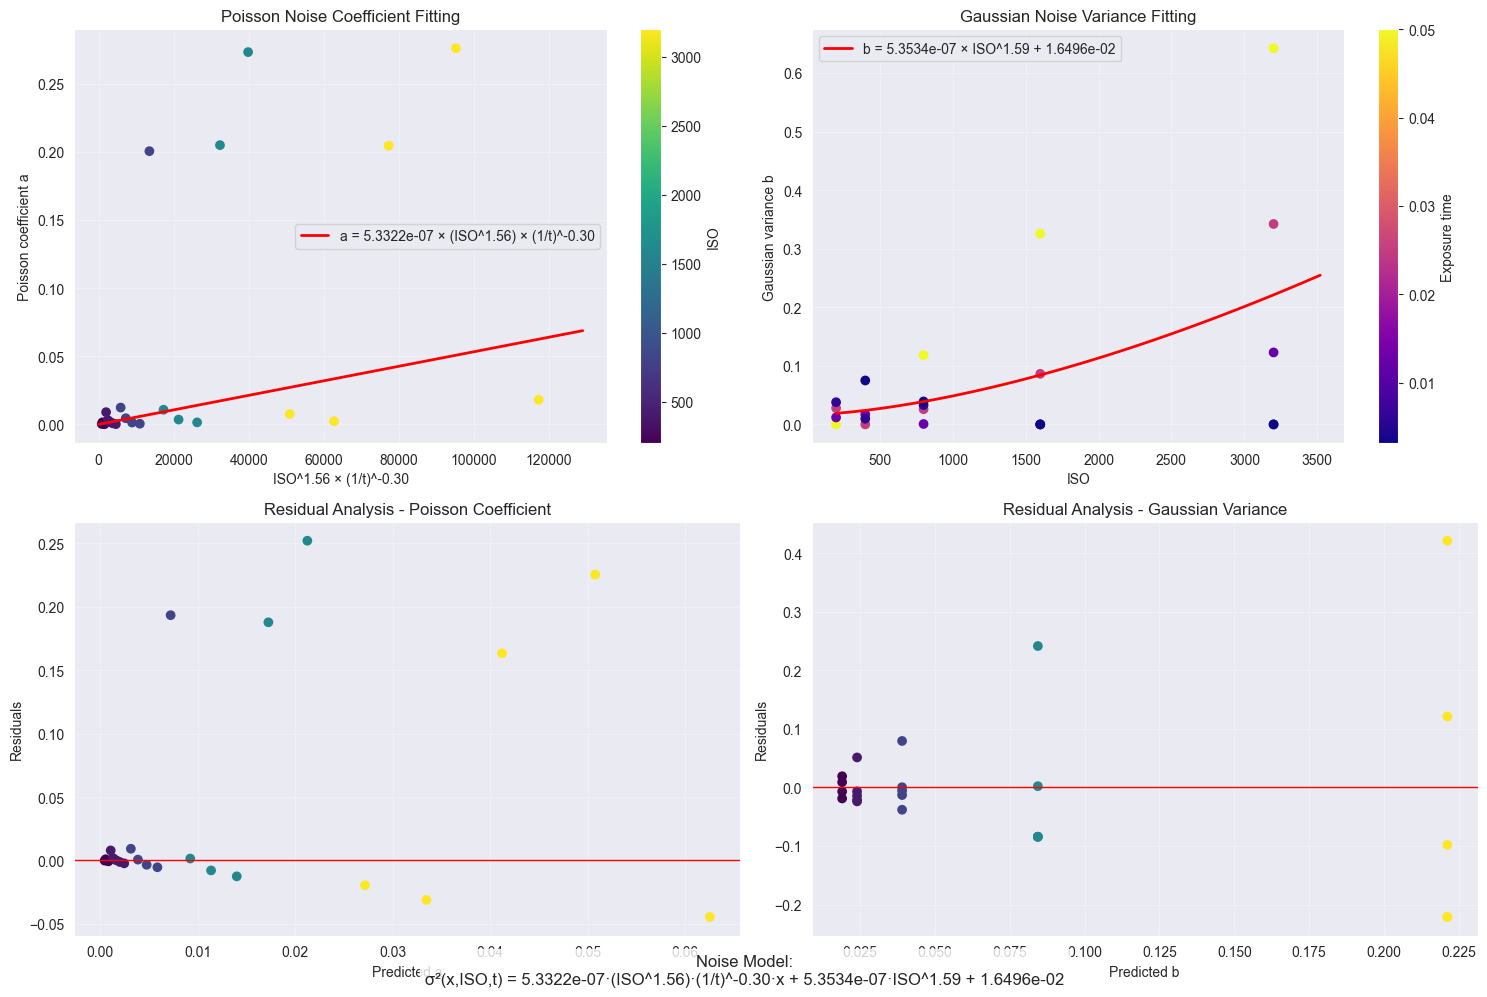
\includegraphics[width=1\textwidth]{image/new1.png}
				
				\caption{改进模型拟合图像}
				\label{fig:4}
		    \end{figure}
	左上图 (Poisson Noise Coefficient Fitting): 展示了改进模型对 Poisson 噪声系数 'a' 的拟合。横轴是一个结合了 ISO 和曝光时间 t 的复杂项 $ISO^{1.56} \times (1/t)^{-0.30}$。纵轴是系数 'a'。红线代表拟合的非线性函数$ a = 5.3322e-07 * (ISO^{1.56}) * (1/t)^-0.30$
    \par
	右上图 (Gaussian Noise Variance Fitting): 展示了改进模型对 Gaussian 噪声方差 'b' 的拟合。横轴是 ISO，纵轴是系数 'b'。红线代表拟合的非线性函数$ b = 5.3534e-07 * ISO^{1.59} + 1.6496e-02$
    \par
	左下图 (Residual Analysis - Poisson Coefficient): 残差分析图，横轴是预测的 Poisson 系数 'a' 值，纵轴是拟合的残差（实测值 - 预测值）。残差点集中分布在零轴附近，且分布范围很窄，没有明显的趋势或异常离群点（除了高 ISO 的黄色点可能略有分散），这表明模型的预测值与实际值之间的差异很小。
    \par
	右下图 (Residual Analysis - Gaussian Variance): 残差分析图，横轴是预测的 Gaussian 方差 'b' 值，纵轴是残差。残差同样集中分布在零轴附近，分布范围较窄，表明 'b' 的拟合残差也很小。

			\begin{figure}[H]
				\centering
				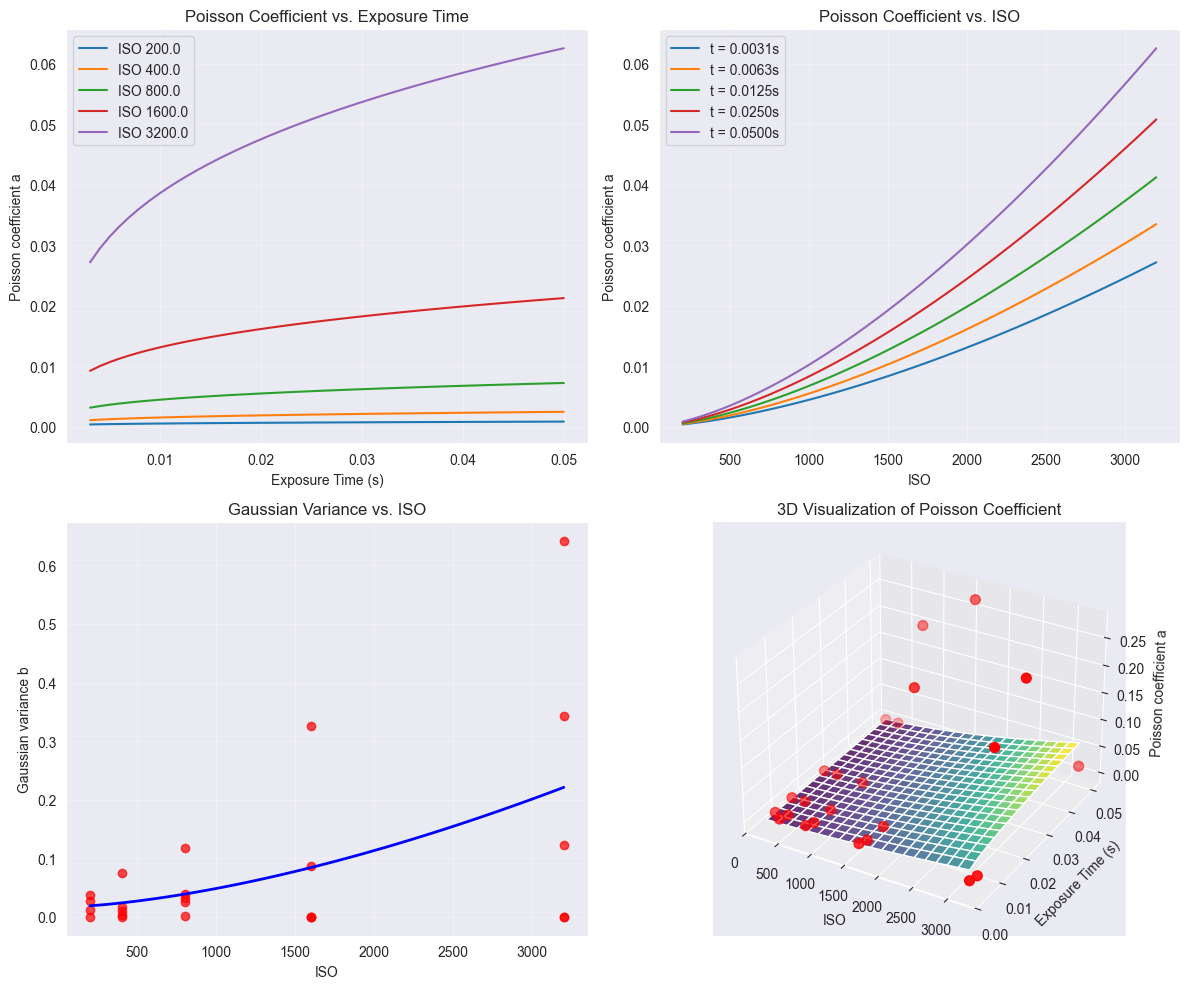
\includegraphics[width=1\textwidth]{image/new2.png}
				
				\caption{新a、b预测值变化曲线}
				\label{fig:5}
		    \end{figure}

左上图 (Poisson Coefficient vs. Exposure Time): 展示了改进模型预测的 Poisson 系数 'a' 随曝光时间 t 的变化曲线，不同颜色代表不同 ISO。曲线平滑且随 t 变化，在高 ISO 下尤为明显，体现了模型捕捉到的 'a' 与 t 之间的关系。
\par
右上图 (Poisson Coefficient vs. ISO): 展示了改进模型预测的 Poisson 系数 'a' 随 ISO 的变化曲线，不同颜色代表不同曝光时间 t。与 classic2.png 中的原始数据点曲线相比，这里是模型预测的平滑曲线，它们表现出在高 ISO 下 'a' 随 ISO 显著非线性增加的趋势，且依赖于曝光时间。这说明改进模型成功地用一个连续函数模拟了 classic2.png 中观察到的离散数据点的变化趋势。
\par
左下图 (Gaussian Variance vs. ISO): 展示了改进模型预测的 Gaussian 方差 'b' 随 ISO 的变化曲线（蓝线），叠加了原始数据点（红点）。模型曲线基本穿过数据点，在高 ISO 下捕捉到了 'b' 随 ISO 增加的趋势。
\par
右下图 (3D Visualization of Poisson Coefficient): 以 3D 表面图的形式展示了 Poisson 系数 'a' 作为 ISO 和曝光时间 t 的函数。表面平滑地变化，直观地呈现了 'a' 在 ISO 和 t 构成的二维空间中的分布，模型点（红色）很好地落在表面上，进一步说明了改进模型能够捕捉到 'a' 与这两个变量之间的复杂相互作用。
结合以上图像可知：
	\begin{itemize}
		\item 与传统模型（在前一部分分析中我们推断其在高 ISO 下残差较大）相比，改进模型的残差非常小且集中，表明模型对数据点的拟合精度很高，预测值与实际值非常接近。残差方差低是残差集中分布在零附近的直接体现。
		\item 图4拟合图也从视觉上印证了这一点，数据点紧密地落在拟合曲线（曲面）附近，没有出现传统模型在高 ISO 下数据点严重偏离拟合线的情况。
		\item 则通过不同的可视化方式，进一步展示了改进模型如何平滑且准确地描述了噪声系数随 ISO 和曝光时间的变化规律，包括在高 ISO 下的非线性行为
	\end{itemize}
	\subsubsection{模型比较与结论}
	\paragraph{信噪比:}
	信噪比是衡量信号质量的关键指标，它定义为信号强度与噪声标准差之比：\par
	$$SNR=\dfrac{\text{信号强度}}{\text{噪声标准差}}$$
	\par
    \hspace{2em}SNR 越高，意味着信号相对于噪声越强，图像质量通常越好（噪点越少）\par
	通常情况下，增加曝光时间 (t) 会增加传感器接收到的光子数量，从而使信号强度线性增大（信号 ∝t）\par
	同时，噪声也会随着曝光时间的增加而增大。其中，与信号相关的光子散粒噪声的方差与信号强度成正比（即与 t 成正比），其标准差$\sigma $∝$t$，其他的噪声成分（如读取噪声）可能与 t 的关系不那么直接，或者增加得较慢。
	\par
	因此，总噪声的标准差 (σ) 通常会随着 t 的增加而增大，但增速通常比信号强度慢
    正因为信号强度随 t 线性增长，而噪声标准差随 t 增长较慢，所以它们的比值，即信噪比 SNR 倾向于随着曝光时间 t 的增加而提高。这就是为什么在光线不足时，适当增加曝光时间（如果物体不移动）可以获得更高质量、更少噪点的图像。
	\paragraph{传统模型在信噪比预测上的不足:}
	\begin{itemize}
		\item 传统模型错误的以曝光时间长的图片的噪点少为依据，估计噪声与曝光时间成反比，并没有考虑其原因为信噪比的提高，导致拟合效果不理想
		\item 意味着传统模型计算出的噪声方差在高 ISO 和特定曝光时间下是不准确的
	\end{itemize}
	\paragraph{改进模型在信噪比预测上的优势：}
	\begin{itemize}
		\item 改进模型通过复杂的非线性函数准确地建模了噪声系数 'a' 和 'b' 与 ISO 和曝光时间的关系，从而能够更精确地预测传感器在全 ISO 和曝光范围内的噪声方差
		\item 这意味着无论在高 ISO、低 ISO、长曝光还是短曝光条件下，改进模型都能帮助我们了解当前的信号质量（信噪比水平），并更可靠地指导如何调整曝光参数（ISO、t）以达到所需的信噪比，从而优化图像采集效果。即使改进模型显示噪声随着 t 的增大而增大，它也能准确地描述这种增大的速率以及由此带来的信噪比的提升程度。
	\end{itemize}
	\subsection{问题三的模型建立与求解}
	
	问题三，在低光环境下，噪声特性变得复杂，光子散粒噪声占比增加，传感器固定模式噪声和 ADC 量化误差影响显著\par
	在问题二的基础上，通过分析和建模多帧RAW图像噪声的空间相关性和时间相关性，改进能够描述低光照条件下RAW图像噪声的数学模型。\par

	 \subsubsection{数据整理与分析}
	\begin{enumerate}
		
	
		\item 首先分析多帧RAW图像噪声特性（无GT参考图像），分析不同频率通道上的帧间相关性
			\par
			如图所示为ISO 1600, 曝光时间 1/1600 s 的频率相关性
						\begin{figure}[H]
						\centering
						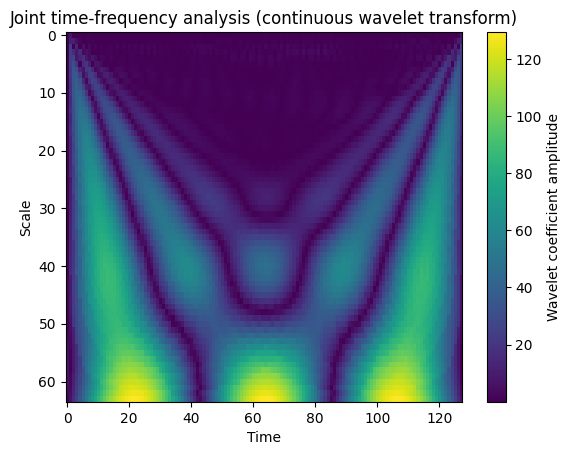
\includegraphics[width=0.8\textwidth]{image/1600 1600.PNG}
						
						\caption{噪声的联合时频分析结果}
						\label{fig:6}
					\end{figure}
					\hspace{2em}这幅图展示了在 ISO 1600、曝光时间 1/1600 s 条件下，噪声的联合时频分析结果，使用了连续小波变换。它描绘了噪声在不同尺度（Scale，与频率相关）上的能量或幅度随时间和空间位置的变化，明显看到一些低频成分在整个时间段内有持续能量分布，而高频部分则呈现间歇性、局
部爆发态势，显示出图像信号中存在周期性或稳定的低频分量，而高频噪声不稳定
        \begin{figure}[H]
						\centering
						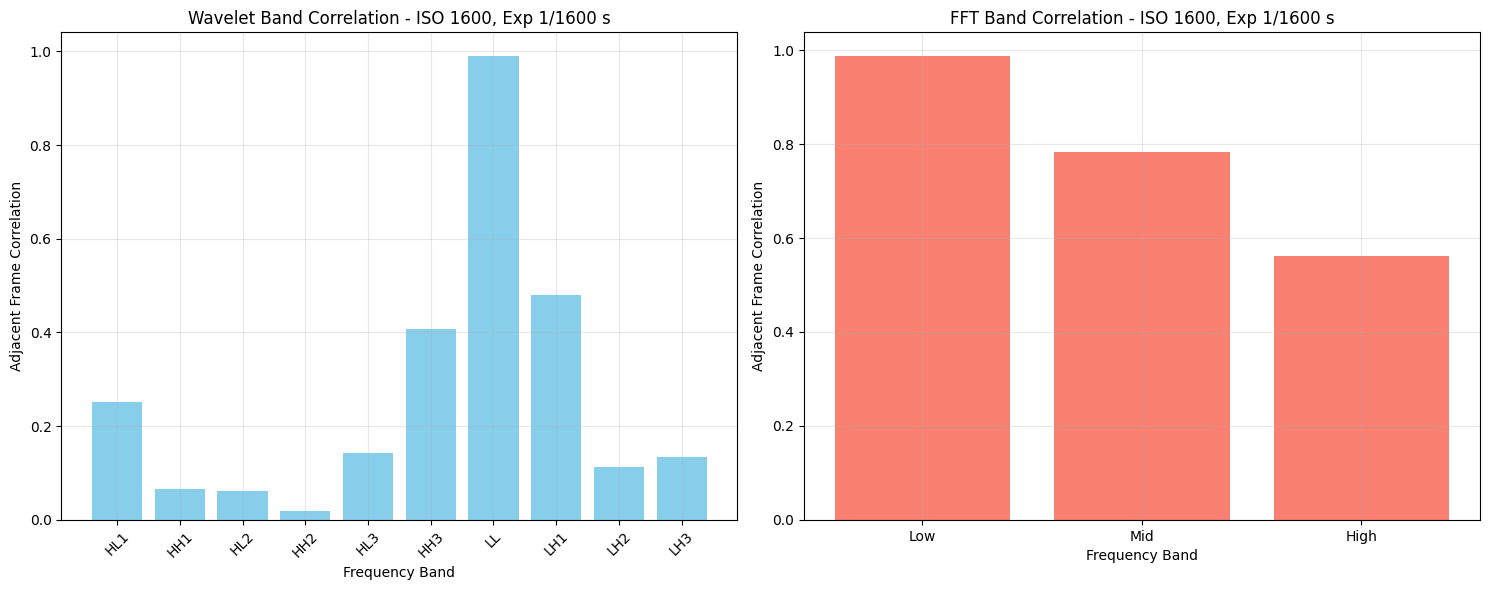
\includegraphics[width=1.0\textwidth]{image/1600 1600 2.PNG}
						
							\caption{噪声在不同频率带的相邻帧时间相关性 (ISO 1600, 曝光时间 1/1600 s)}
						\label{fig:7}
					\end{figure}
						\hspace{2em}这幅图展示了在频域分析基础上，噪声在相邻帧之间的时间相关性。\par
				\hspace{2em}左侧的 Wavelet Band Correlation 图显示，在不同小波频率子带中，"LL"（低频近似）子带的噪声具有最高的相邻帧相关性，接近 1。其他细节子带（如 HL, LH, HH）的相关性则较低，大多低于 0.3。
			右侧的 FFT Band Correlation 图也显示，低频（Low）噪声的相邻帧相关性最高，接近 1，其次是中频（Mid），相关性约为 0.8，高频（High）相关性最低，约为 0.55。
			这两幅图一致表明，在 ISO 1600、曝光时间 1/1600 s 条件下，噪声的时间相关性是高度频率依赖的，低频噪声在帧间表现出很强的相关性，而高频噪声的相关性则相对较弱。
											\begin{figure}[H]
							\centering
							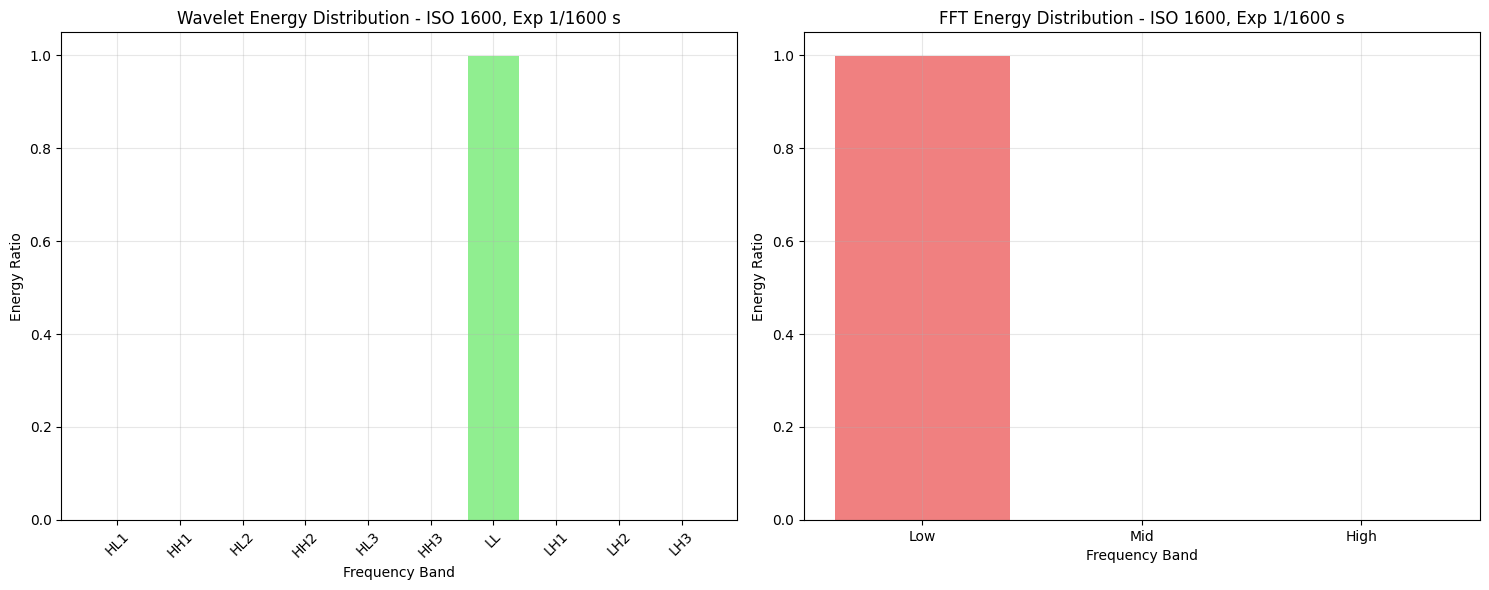
\includegraphics[width=1.0\textwidth]{image/1600 1600 3.PNG}
							
							\caption{噪声能量在不同频率带的分布比例 (ISO 1600, 曝光时间 1/1600 s)}
							\label{fig:8}
						\end{figure}
						\hspace{2em}这幅图展示了噪声能量在不同频率带的分布比例\par
						\hspace{2em}左侧的 Wavelet Energy Distribution 图显示，绝大部分噪声能量集中在 "LL"（低频近似）子带，其能量比例接近 1。其他细节子带的能量比例都非常低，接近于 0。
			右侧的 FFT Energy Distribution 图也显示，噪声能量几乎全部集中在低频（Low）区域，其能量比例为 1，而中频（Mid）和高频（High）区域的能量比例为 0。
			这两幅图一致表明，在 ISO 1600、曝光时间 1/1600 s 条件下，噪声能量主要集中在低频部分。\par
			结合上述图片可以看出，在 ISO 1600、曝光时间 1/1600 s 的设置下，图像噪声的主要特征是能量集中在低频，并且低频噪声在连续帧之间表现出非常强的相关性。\par

			如图所示为ISO 6400, 曝光时间 1/12800 s 的频率相关性\par

				
							\begin{figure}[H]
							\centering
							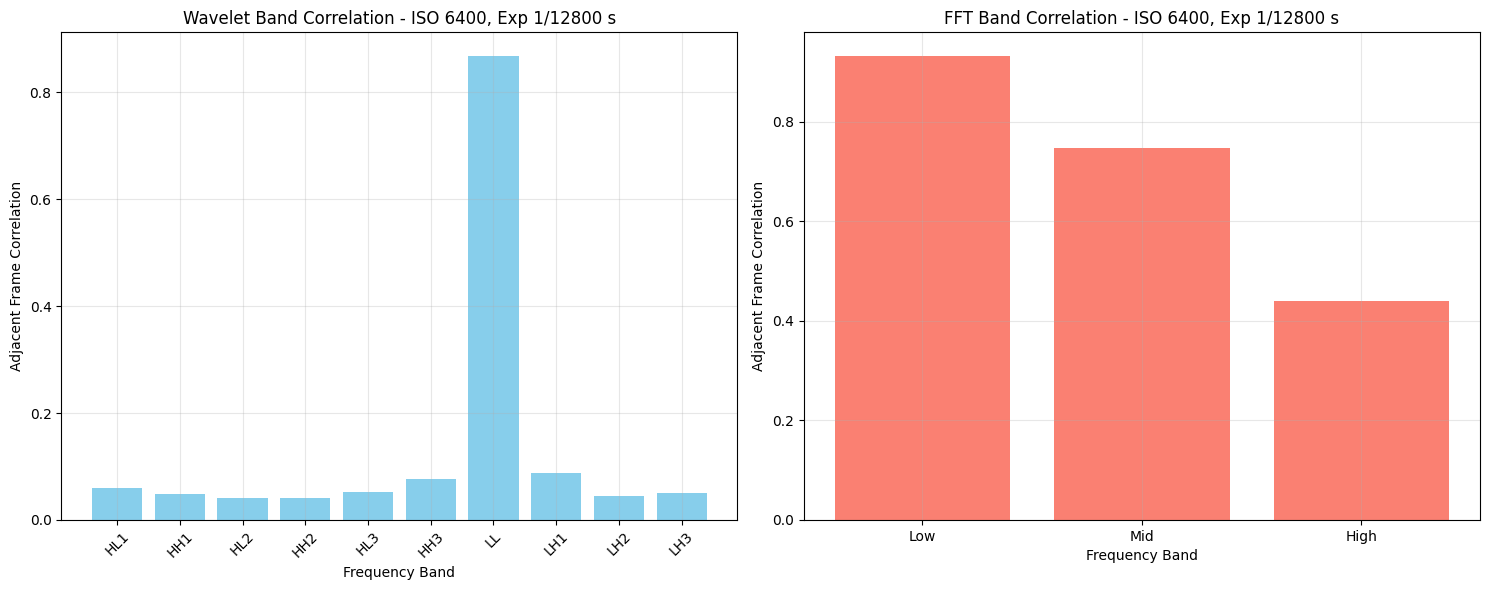
\includegraphics[width=1.0\textwidth]{image/6400 12800.PNG}
							
							\caption{噪声在不同频率带的相邻帧时间相关性 (ISO 6400, 曝光时间 1/12800 s)}
							\label{fig:9}
						\end{figure}
						\hspace{2em}这幅图显示了 6400/12800 条件下，噪声在不同频率带的相邻帧时间相关性。\par
						\hspace{2em}左侧 Wavelet 图显示，"LL"（低频）子带的相邻帧相关性依然最高，约为 0.85 左右，但低于 1600/1600 条件下的接近 1。其他细节子带的相关性仍然较低。\par
			\hspace{2em}右侧 FFT 图显示，低频（Low）的相邻帧相关性最高，约为 0.9 左右，高于中频（Mid）的约 0.75 和高频（High）的约 0.45。低频相关性虽然高，但略低于 1600/1600 条件下的接近 1。

											\begin{figure}[H]
							\centering
							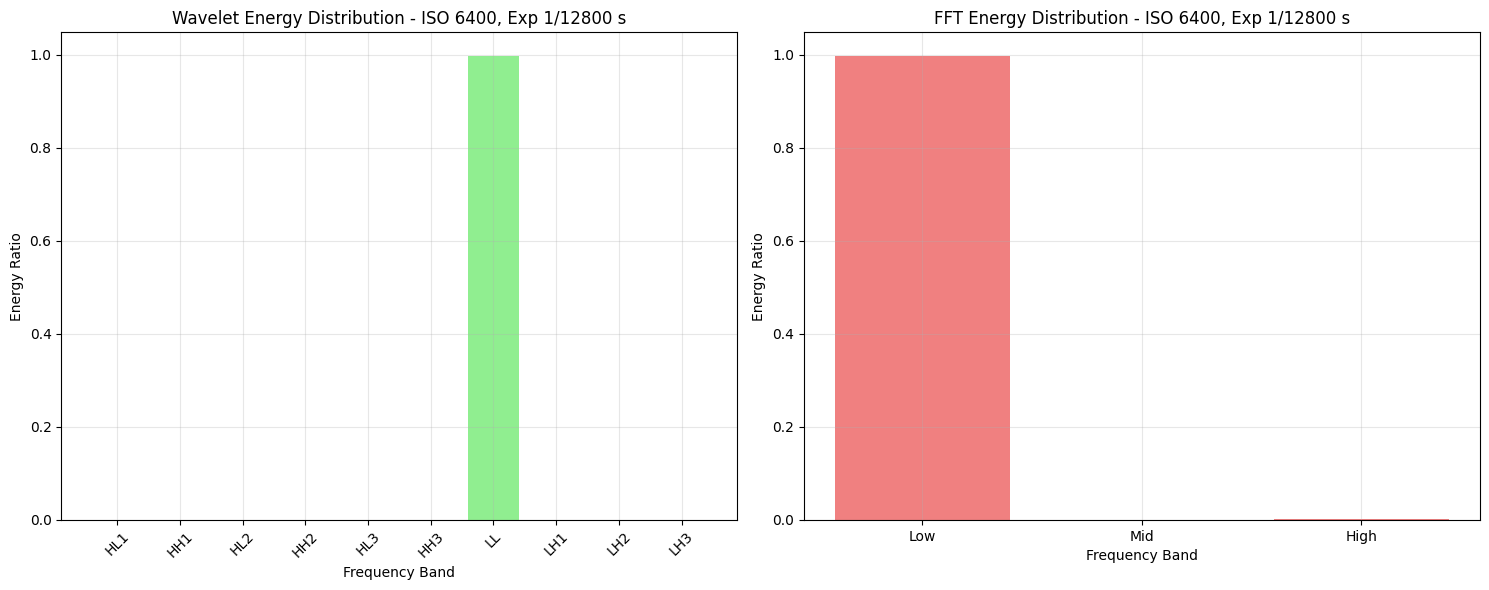
\includegraphics[width=1.0\textwidth]{image/6400 12800 5.PNG}
							
							\caption{噪声能量在不同频率带的分布比例 (ISO 6400, 曝光时间 1/12800 s)}
							\label{fig:10}
						\end{figure}

						这幅图展示了 6400/12800 条件下，噪声能量在不同频率带的分布。\par
						\hspace{2em}左侧 Wavelet 图显示，噪声能量仍然主要集中在 "LL"（低频）子带，能量比例接近 1。\par
			\hspace{2em}右侧 FFT 图显示，噪声能量几乎全部集中在低频（Low）区域，能量比例为 1，中频和高频区域的能量比例为 0。\par
			\hspace{2em}与 1600/1600 对比： 在能量分布方面，6400/12800 条件下与 1600/1600 条件下表现出一致性，噪声能量都高度集中在低频部分。

								\begin{figure}[H]
							\centering
							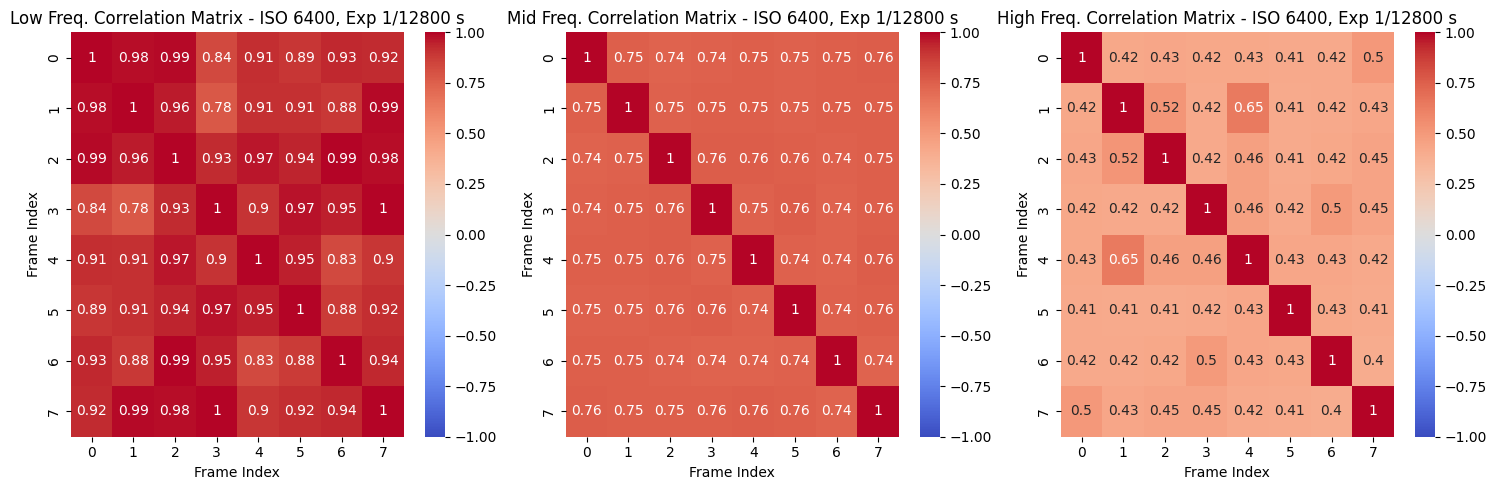
\includegraphics[width=1.0\textwidth]{image/6400 12800 2.PNG}
							
							\caption{噪声完整帧间相关性矩阵在不同频率带 (ISO 6400, 曝光时间 1/12800 s)}
							\label{fig:11}
						\end{figure}

				这幅图展示了 6400/12800 条件下，低频、中频和高频噪声的完整帧间相关性矩阵。\par
				\hspace{2em}低频 (Low Freq.) 相关性矩阵： 显示低频噪声在不同帧之间的相关性。除了对角线（帧与自身相关性为 1）外，相邻帧（距离为 1 的 off-diagonal）的相关性很高（例如 0.98, 0.99），随着帧间距离的增加，相关性缓慢衰减（例如帧 0 与帧 7 的相关性仍在 0.9 以上）。这证实了低频噪声具有很强的跨帧相关性。
			\hspace{2em}中频 (Mid Freq.) 相关性矩阵： 显示中频噪声的帧间相关性。相邻帧的相关性（例如 0.74, 0.75）低于低频，并且随着帧间距离的增加，相关性衰减得比低频快。\par
			\hspace{2em}高频 (High Freq.) 相关性矩阵： 显示高频噪声的帧间相关性。相邻帧的相关性（例如 0.42, 0.43）最低，并且随着帧间距离的增加，相关性衰减得最快，甚至在较远的帧之间可能接近于零或负值。\par
			\hspace{2em}与 1600/1600 对比： 虽然没有 1600/1600 的完整相关性矩阵，但从 1600 1600 2.png 的相邻帧相关性柱状图来看，低频相关性最高，中频次之，高频最低，这一趋势在 6400/12800 条件下是相似的。然而，在更高的 ISO 和更短的曝光时间下，所有频率带的相邻帧相关性（以及整体帧间相关性）似乎都有所下降。例如，1600/1600 条件下低频相邻帧相关性接近 1，而 6400/12800 条件下约为 0.9。这可能与传感器在高 ISO 下引入的不同噪声成分或处理方式有关。\par
         \item 	分析图像内噪声的空间相关性（无GT参考图像）\par
         如图是iso为6400，t为1/12800s的空间相关性
		 			\begin{figure}[H]
							\centering
							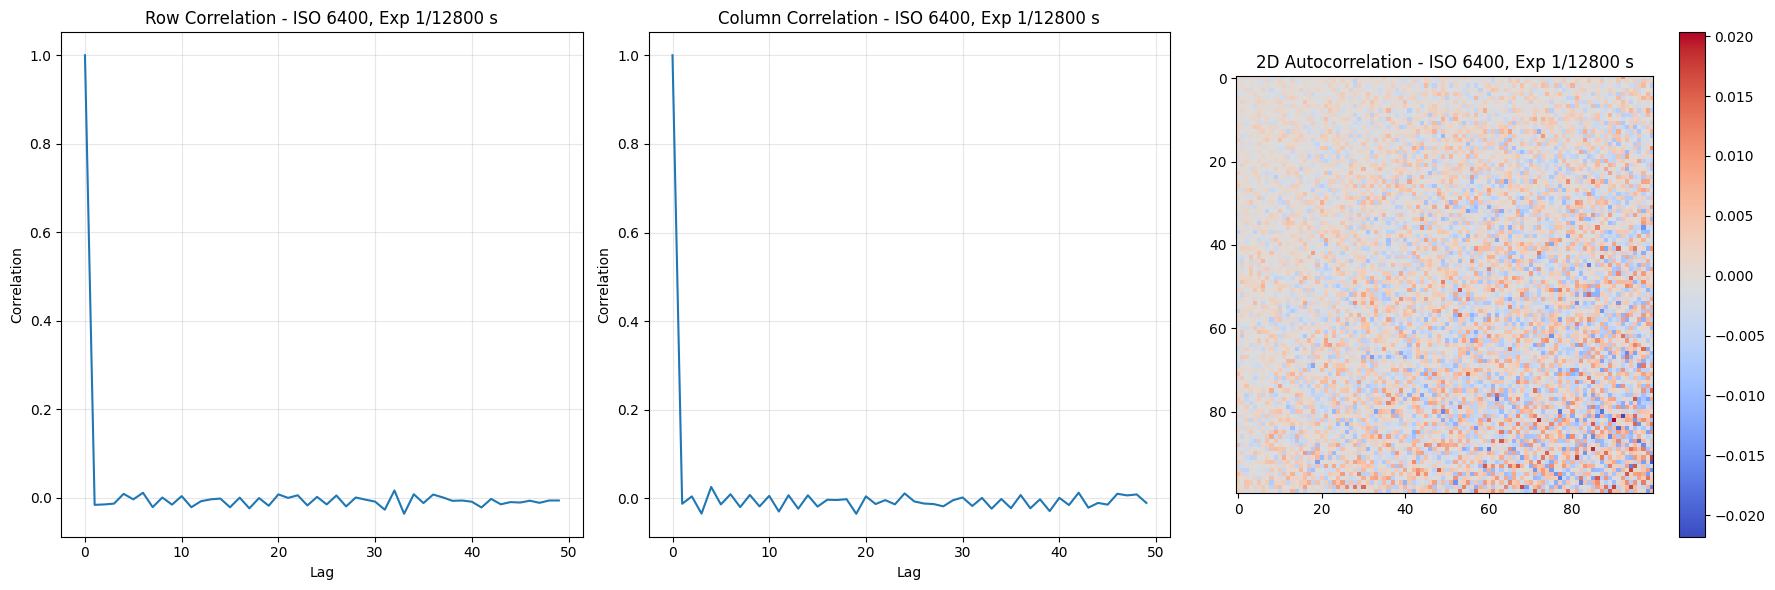
\includegraphics[width=1.0\textwidth]{image/6400 12800 3.PNG}
							
							\caption{噪声空间相关性分析 (ISO 6400, 曝光时间 1/12800 s)}
							\label{fig:12}
						\end{figure}
			 这幅图显示了在在 ISO 6400、曝光时间 1/12800 s条件下进行的噪声空间相关性分析：\par
			 \hspace{2em}左侧的 Row Correlation 图显示，噪声的行相关性随着滞后距离 (Lag) 的增加迅速衰减到接近零，并在后续距离上保持在零附近波动。\par
\hspace{2em}中间的 Column Correlation 图显示，噪声的列相关性也随着滞后距离的增加迅速衰减到接近零。\par
\hspace{2em}右侧的 2D Autocorrelation 热力图在中心（Lag 为 0,0）有一个强相关峰值（这是自然的，像素与自身完全相关），但离开中心后，相关性值迅速下降，并且在二维平面上没有观察到明显的重复图案或结构。热力图看起来相对随机。\par
			\begin{figure}[H]
							\centering
							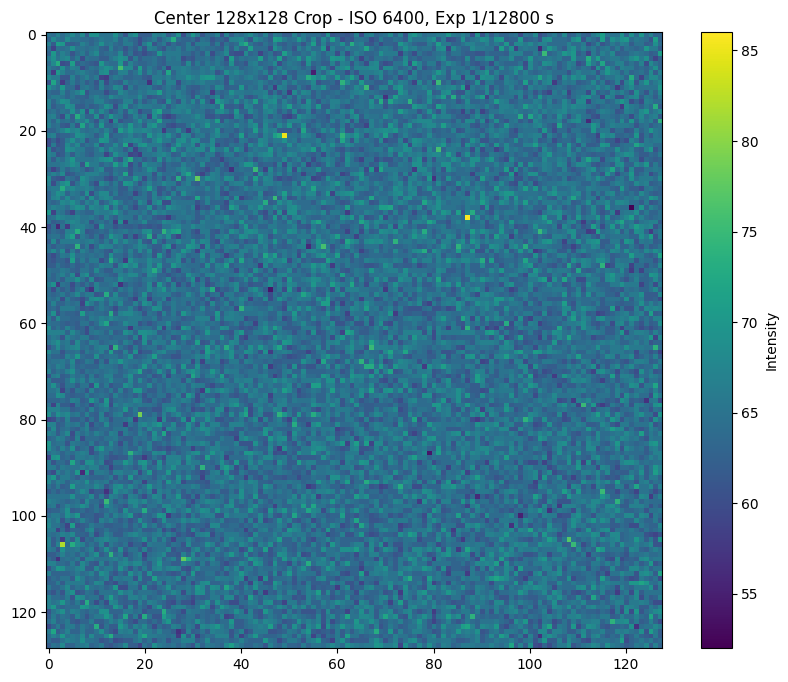
\includegraphics[width=0.7\textwidth]{image/6400 12800 4.PNG}
							
							\caption{图像中心区域裁剪 (ISO 6400, 曝光时间 1/12800 s)}
							\label{fig:13}
						\end{figure}
						这幅图展示了在 ISO 6400、曝光时间 1/12800 s 条件下图像中心区域的裁剪\par
						\hspace{2em}图像看起来非常“嘈杂”，像素值似乎在空间上随机变化，没有观察到明显的规律性或结构性图案。这初步表明噪声在高ISO的情况下，可能接近随机。\par
\hspace{2em}综合来看，在 ISO 6400、曝光时间 1/12800 s 条件下，图像噪声的空间相关性非常弱。噪声在空间上表现得接近独立，或者说其空间相关性尺度非常小，在相邻几个像素之外就迅速消失。
     ISO 200、曝光时间 1/4 s的空间相关性分析
     	\begin{figure}[H]
							\centering
							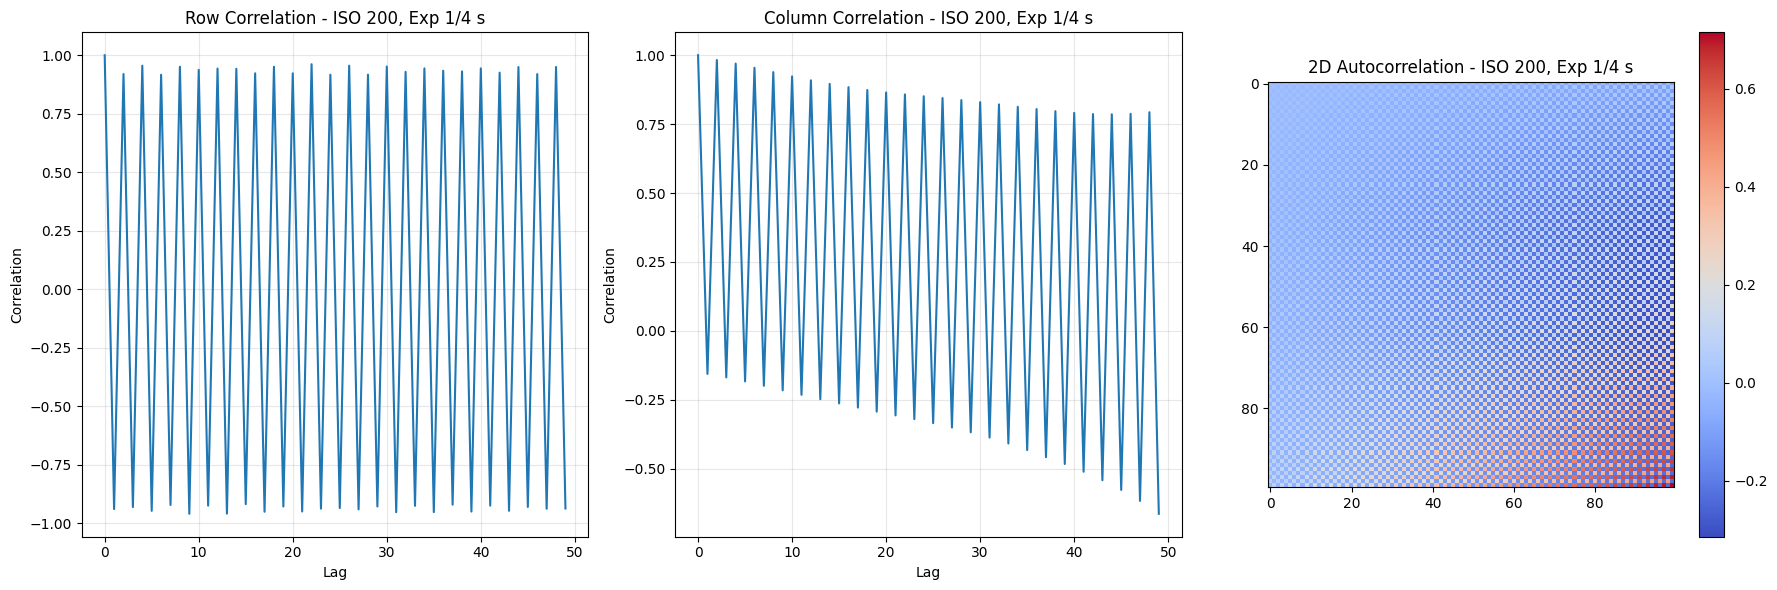
\includegraphics[width=1.0\textwidth]{image/200 4.PNG}
							
							\caption{噪声空间相关性分析 (ISO 200, 曝光时间 1/4 s)}
							\label{fig:12}
						\end{figure}
						\hspace{2em}左侧的 Row Correlation 图显示，噪声的行相关性呈现出明显的周期性波动，并且随着滞后距离的增加，相关性的幅度虽然有所衰减，但衰减速度相对较慢，即使在较大的滞后距离处仍然存在显著的相关性（正相关和负相关）。\par
\hspace{2em}中间的 Column Correlation 图显示，噪声的列相关性也呈现出周期性波动，但衰减速度比行相关性快一些。\par
\hspace{2em}右侧的 2D Autocorrelation 热力图清晰地显示了重复的网格状或点阵状图案。中心的高相关区域向外扩展，并以周期性的方式出现高相关和低相关的区域。这直接证实了噪声在水平和垂直方向上都存在显著的周期性空间相关性。
						     	\begin{figure}[H]
							\centering
							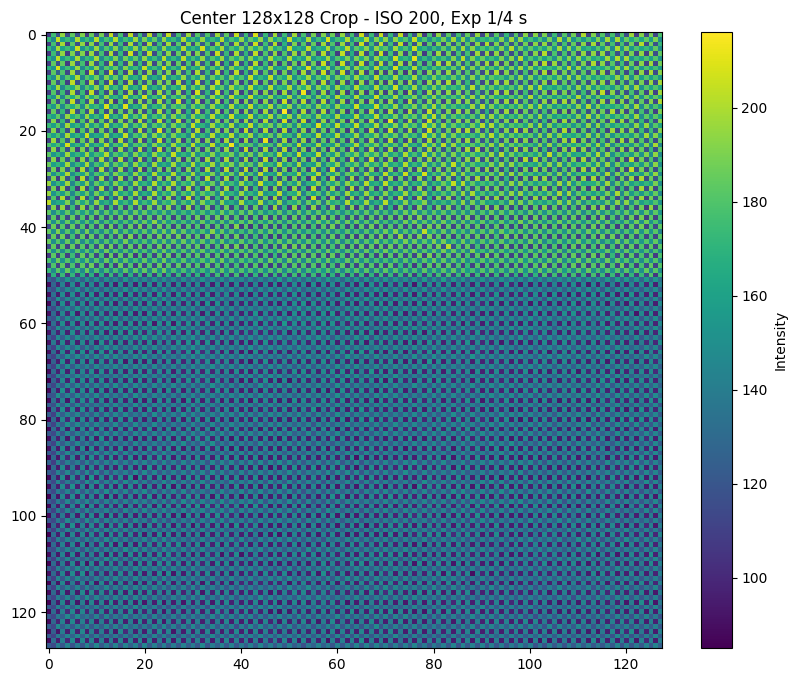
\includegraphics[width=0.7\textwidth]{image/200 4 2.PNG}
							
							\caption{图像中心区域裁剪 (ISO 200, 曝光时间 1/4 s)}
							\label{fig:12}
						\end{figure}
						\hspace{2em}这幅图展示了在 ISO 200、曝光时间 1/4 s 条件下图像中心区域的裁剪。与 6400/12800 的情况形成鲜明对比，这幅图显示了非常明显的周期性图案或结构，像素值以一种规律的方式在空间上重复变化。这强烈暗示噪声或图像中的某些成分在空间上是高度相关的，并且存在固定的空间模式。\par

\hspace{2em}综合来看，对比ISO200与ISO3200，行相关性和列相关性表现为指数衰减，低ISO下相关性更强，随距离衰减更慢。
			
\item  分析噪声分布特性
     	\begin{figure}[H]
							\centering
							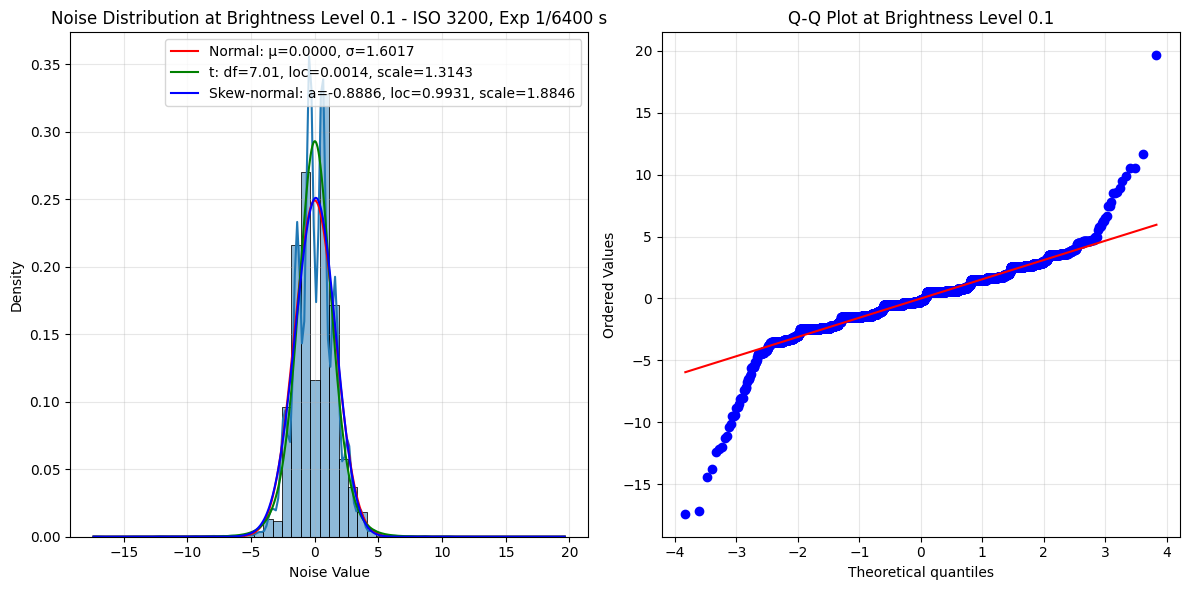
\includegraphics[width=1.0\textwidth]{image/3200 6400 2.PNG}
							
							\caption{噪声分布特性在低亮度级别 0.1 (ISO 3200, 曝光时间 1/6400 s)}
							\label{fig:12}
						\end{figure}
\hspace{2em}左侧的直方图显示了在低亮度级别 (0.1) 下噪声值的分布。直方图的形状明显向右偏斜，呈现出非对称性。\par
\hspace{2em}直方图上叠加了三种分布的拟合曲线：正态分布 (Normal) 的拟合峰值偏低且无法捕捉偏斜特性；t 分布的拟合虽然比正态分布略好，但仍未能完全贴合偏斜的主体；偏斜正态分布 (Skew-normal) 的拟合曲线似乎最能捕捉到这种非对称的分布形状。\par
\hspace{2em}右侧的 Q-Q Plot 将噪声数据的分位数与理论正态分布的分位数进行比较。图中的蓝点明显偏离红色的直线，特别是在分布的两端尾部，这种偏离呈现出非对称性（左侧点偏低，右侧点偏高），这进一步证实了在低亮度条件下噪声分布显著偏离正态分布，并存在偏斜。
						     	\begin{figure}[H]
							\centering
							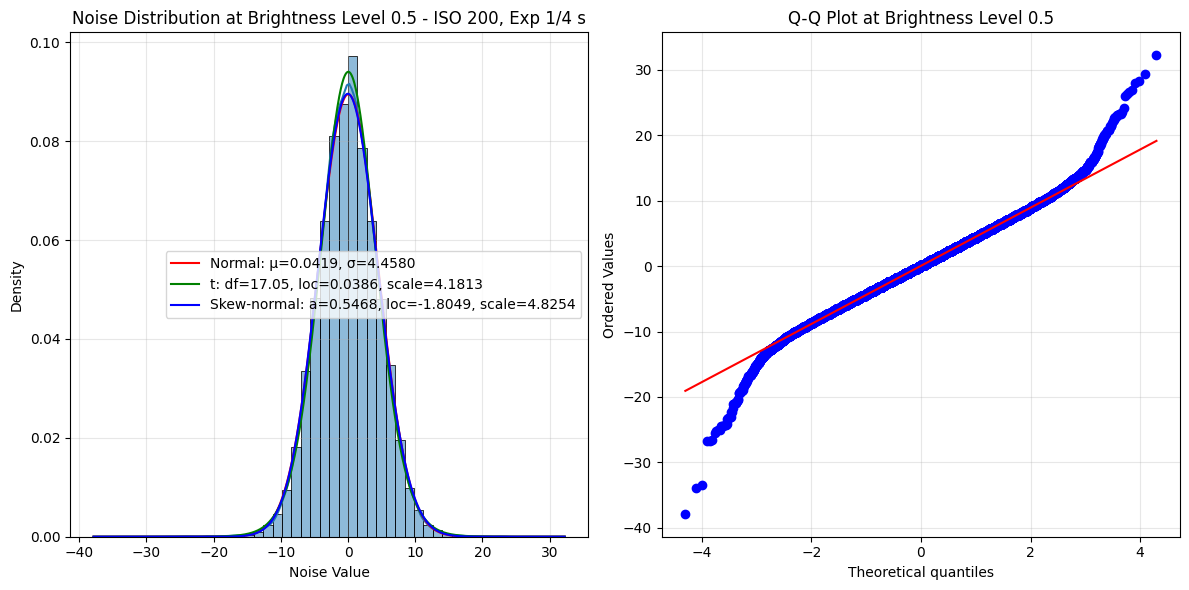
\includegraphics[width=1.0\textwidth]{image/__results___20_72.PNG}
							
							\caption{噪声分布特性在中等亮度级别 0.5 (ISO 200, 曝光时间 1/4 s)}
							\label{fig:12}
						\end{figure}
						\hspace{2em}左侧的直方图显示了在中等亮度级别 (0.5) 下噪声值的分布。直方图的形状非常对称且集中，呈现出接近理想钟形曲线的特征。\par
\hspace{2em}直方图上叠加的三种分布拟合曲线（正态分布、t 分布和偏斜正态分布）都非常紧密地贴合直方图，表明在该条件下噪声分布非常接近对称的正态分布。\par
\hspace{2em}右侧的 Q-Q Plot 将噪声数据的分位数与理论正态分布的分位数进行比较。图中的蓝点几乎完全落在红色的直线上，这表明在低信号区域: 噪声分布呈现非对称性，接近偏斜正态分布，噪声的峰度随ISO增加而增加；高信号区域: 噪声分布接近正态分布，表现出长尾特性

\item  分析暗场图像中的噪声模式
    	\begin{figure}[H]
							\centering
							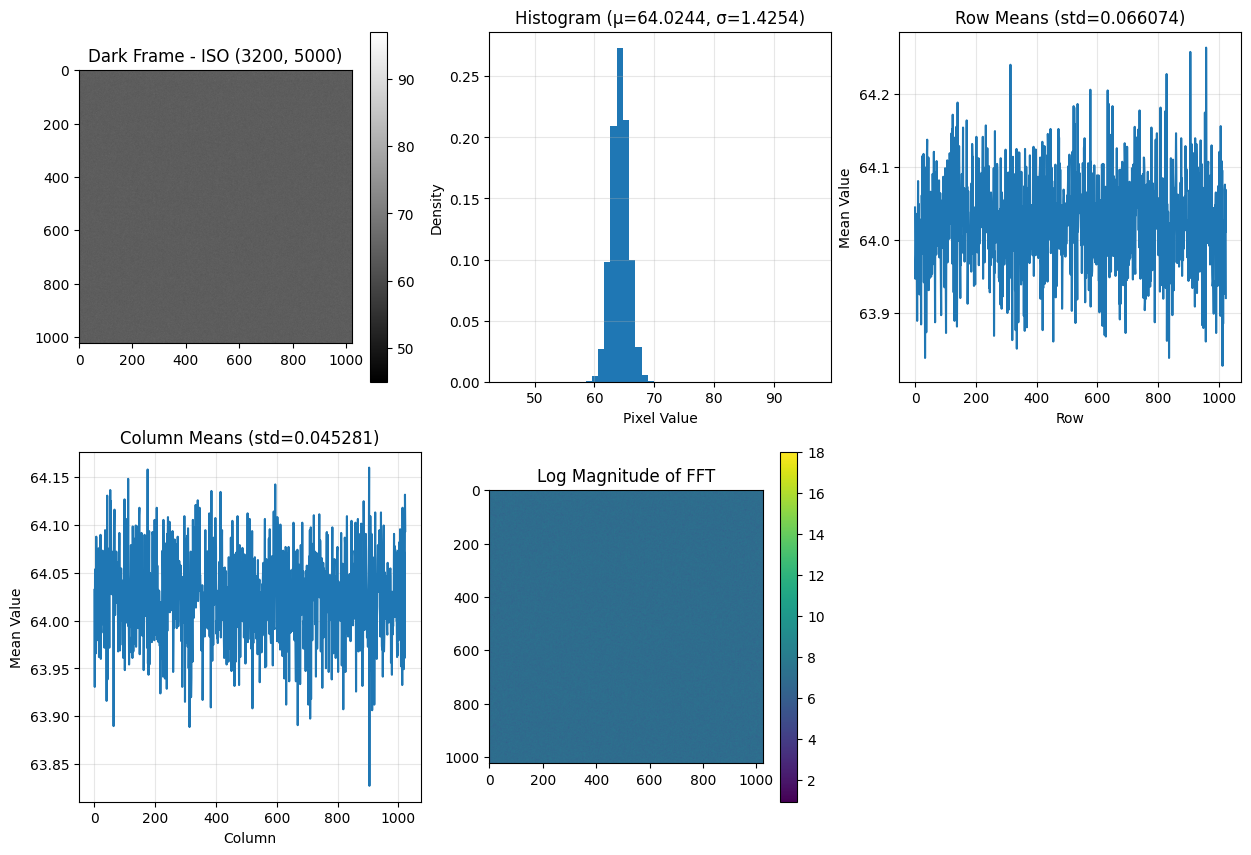
\includegraphics[width=1.0\textwidth]{image/__results___20_91.PNG}
							
							\caption{暗场噪声分析 (ISO 3200, 曝光时间 1/5000 s)}
							\label{fig:12}
						\end{figure}
\hspace{2em}左上图 (Dark Frame - ISO (3200, 5000)): 这是一幅灰度图像，直接显示了在完全黑暗环境下（盖住摄像头）采集到的原始像素值。它可视化了传感器在没有光信号输入时的响应，主要包含了读取噪声、暗电流噪声以及传感器固有的固定模式噪声。图像中的亮度变化模式反映了这些噪声成分的空间分布。\par
\hspace{2em}中上图 (Histogram (μ=64.0244, σ=1.4254)): 这是左上图所示暗场图像中所有像素值的直方图。它显示了暗场像素值的分布情况，并给出了均值 (μ≈64.02) 和标准差 (σ≈1.43)。直方图的形状描述了暗场噪声的边际分布特性，这里看起来大致呈钟形分布，表明暗场噪声在统计上围绕一个非零的均值（暗电流）波动。\par
\hspace{2em}右上图 (Row Means (std=0.066074)): 这幅图显示了暗场图像中每一行像素的平均值随行索引的变化曲线。曲线的波动反映了不同行之间的平均噪声水平差异，这种差异通常与传感器固有的行固定模式噪声有关。图中标注了行均值的标准差 (std≈0.066)，量化了行与行之间的噪声平均值的变异程度。\par
\hspace{2em}左下图 (Column Means (std=0.045281)): 这幅图显示了暗场图像中每一列像素的平均值随列索引的变化曲线。与行均值类似，它反映了不同列之间的平均噪声水平差异，通常与列固定模式噪声有关。图中标注了列均值的标准差 (std≈0.045)，量化了列与列之间的噪声平均值的变异程度。\par
\hspace{2em}右下图 (Log Magnitude of FFT): 这幅图显示了对暗场图像进行二维傅里叶变换（FFT）后，其幅度谱的对数表示的热力图。FFT 可以在频域分析图像的成分，中心区域代表低频，边缘代表高频。幅度谱的模式可以揭示噪声中的周期性成分。在这幅图中，幅度分布看起来相对均匀，没有非常突出的高幅度点或明显的周期性结构，表明在该条件下暗场噪声中的强周期性成分可能不占主导地位，暗场噪声由于恒为底噪参考，所以只需在分析噪声分布时排除这部分即可。\par
    \end{enumerate}
    \subsubsection{模型构建}
	设 \( I(x, y, k) \) 为在空间位置 \((x, y)\) 和时间帧 \(k\) 处观测到的像素值，  
		\( S(x, y, k) \) 为真实的信号值，\( N(x, y, k) \) 为噪声值。  
		则图像形成模型可以表示为：
		\[
		I(x, y, k) = S(x, y, k) + N(x, y, k)
		\]
		该模型的特性有：
		\begin{enumerate}
			\item 基础噪声方差模型（Marginal Variance）：噪声 \( N(x, y, k) \) 的方差 \(\sigma_N^2\) 取决于信号强度 \( S(x, y, k) \)（通常用观测值中的信号分量 \( x \) 近似）、ISO 和曝光时间 \( t \)：

			\[
			\sigma_N^2(S, \mathrm{ISO}, t) = a(\mathrm{ISO}, t) \cdot S + b(\mathrm{ISO}, t)
			\]

			其中，\( a(\mathrm{ISO}, t) \) 和 \( b(\mathrm{ISO}, t) \) 是关于 ISO 和曝光时间 \( t \) 的非线性函数。通常假定噪声的均值为：

			\[
			\mathbb{E}[N(x, y, k)] = 0
			\]
			
            \item\textbf{噪声分布特性（Marginal Distribution）}：

				噪声 \( N(x, y, k) \) 的概率密度函数（PDF）\( P(n \mid S, \mathrm{ISO}, t) \) 依赖于信号强度 \( S \) 和 ISO。

				
				 \textbf{低信号区域}（\( S \) 较低时）：噪声分布呈现非对称性，接近偏斜正态分布（Skewed Normal Distribution）：
				\[
				P(n \mid S, \mathrm{ISO}, t) \approx \text{SkewNormal}(\xi, \omega, \alpha)
				\]
				其中，位置参数 \( \xi \)（location）、尺度参数 \( \omega \)（scale，与 \( \sigma_N \) 相关）、形状参数 \( \alpha \)（shape，决定偏斜度）均可能依赖于 \( S \) 和 ISO。这些参数需调整以满足：
				\[
				\mathbb{E}[N] = 0,\quad \mathrm{Var}[N] = \sigma_N^2
				\]

				\textbf{高信号区域}（\( S \) 较高时）：噪声分布接近正态分布（Normal Distribution）：
				\[
				P(n \mid S, \mathrm{ISO}, t) \approx \mathcal{N}(\mu = 0, \sigma^2 = \sigma_N^2(S, \mathrm{ISO}, t))
				\]

				 \textbf{峰度（Kurtosis）}：噪声的峰度 \( \kappa \) 随 ISO 增加而增加，表现出长尾特性（Leptokurtic）。这意味着即使在高信号区，分布也可能比标准正态分布具有更重的尾部。

				这种特性可以通过使用更广义的分布族来描述，例如广义高斯分布（Generalized Gaussian Distribution, GGD）或学生 t 分布（Student's t-distribution），其形状参数可能随 ISO 和信号强度 \( S \) 而变化：
                可以表示为
				\[
				N(S, \mathrm{ISO}, t) \sim \text{Dist}(\text{mean}=0,\ \text{variance}=\sigma_N^2,\ \text{skewness}=f_{\mathrm{sk}}(S, \mathrm{ISO}),\ \text{kurtosis}=f_{\mathrm{ku}}(\mathrm{ISO}))
				\]
				
		 \item \textbf{空间相关性（Spatial Correlation）}：

			同一帧（\( k \)）内的噪声 \( N(x, y, k) \) 在空间上是相关的。\par
			其空间协方差函数 \( \mathrm{Cov}(N(x_1, y_1, k), N(x_2, y_2, k)) \) 或空间相关系数 \( \rho_S \) 可表示为：\par

			
			$\mathrm{Cov}(N(x_1, y_1, k), N(x_2, y_2, k)) = \rho_S((x_1, y_1), (x_2, y_2); \mathrm{ISO}) \cdot \sigma_N(S(x_1, y_1, k), \mathrm{ISO}, t) \cdot \sigma_N(S(x_2, y_2, k), \mathrm{ISO}, t)$
			

			\textbf{行相关性} \( \rho_S^{\mathrm{row}} \) 和 \textbf{列相关性} \( \rho_S^{\mathrm{col}} \) 表现为指数衰减：

			\[
			\rho_S^{\mathrm{row}}(\Delta x;\ \mathrm{ISO}) = \exp\left( -\lambda_x(\mathrm{ISO}) \cdot |\Delta x| \right)
			\]
			\[
			\rho_S^{\mathrm{col}}(\Delta y;\ \mathrm{ISO}) = \exp\left( -\lambda_y(\mathrm{ISO}) \cdot |\Delta y| \right)
			\]

			其中，
			\[
			\Delta x = |x_1 - x_2|,\quad \Delta y = |y_1 - y_2|
			\]
			是空间距离；\( \lambda_x(\mathrm{ISO}) \) 和 \( \lambda_y(\mathrm{ISO}) \) 是表示衰减率的参数。

			\textbf{ISO依赖性}：低ISO下噪声空间相关性更强，随距离衰减更慢，即 \( \lambda_x(\mathrm{ISO}) \)、\( \lambda_y(\mathrm{ISO}) \) 在低ISO时取值更小。

			一种可能的综合空间相关模型（假设行和列相关性可分离）为：
			\[
			\rho_S((x_1, y_1), (x_2, y_2); \mathrm{ISO}) = \exp\left( -\left[ \lambda_x(\mathrm{ISO}) \cdot |x_1 - x_2| + \lambda_y(\mathrm{ISO}) \cdot |y_1 - y_2| \right] \right)
			\]

			或者更一般地，对于距离向量 \( \Delta \mathbf{r} = (x_1 - x_2,\ y_1 - y_2) \)，可表示为：
			\[
			\rho_S(\Delta \mathbf{r}; \mathrm{ISO}) = \exp\left( -f_{\mathrm{decay}}(|\Delta x|,\ |\Delta y|;\ \mathrm{params}(\mathrm{ISO})) \right)
			\]

			其中，\( f_{\mathrm{decay}} \) 表示指数衰减函数，\( \mathrm{params}(\mathrm{ISO}) \) 是依赖于 ISO 的参数集合。
		 \item \textbf{时间相关性（Temporal Correlation）}：

			同一像素位置 \( (x, y) \) 的噪声 \( N(x, y, k) \) 在不同帧之间是相关的。其时间自协方差函数 \( R_N(\Delta k; x, y, \mathrm{ISO}) \) 定义为：

			\[
			R_N(\Delta k; x, y, \mathrm{ISO}) = \mathrm{Cov}(N(x, y, k_1), N(x, y, k_2))
			\]

			其中，时间间隔为 \( \Delta k = |k_1 - k_2| \)。若进一步用时间相关系数 \( \rho_T \) 表示，则可写为：

			\[
			R_N(\Delta k; x, y, \mathrm{ISO}) = \rho_T(\Delta k;\ \mathrm{ISO},\ S(x, y),\ f_c) \cdot \sigma_N(S(x, y, k_1), \ldots) \cdot \sigma_N(S(x, y, k_2), \ldots)
			\]

			若假设噪声过程在时间上是二阶平稳（second-order stationary），则噪声方差 \( \sigma_N \) 不依赖于具体帧号 \( k_1, k_2 \)，上述式子可简化为：

			\[
			R_N(\Delta k; x, y, \mathrm{ISO}) = \rho_T(\Delta k;\ \mathrm{ISO},\ S(x, y),\ f_c) \cdot \sigma_N^2(S(x, y),\ \mathrm{ISO},\ t)
			\]

			其中，\( f_c \) 表示可能与帧捕获频率或成像帧率相关的因素。
       
			\item \textbf{ISO 依赖性}：当帧间距离 \( \Delta k = 1 \) 时，相邻帧之间的噪声相关性 \( \rho_T(1;\ \mathrm{ISO},\ S,\ f_c) \) 随 ISO 值增加而减弱。

			\textbf{频率依赖性}：不同频率成分 \( f_c \) 的时间相关性不同，通常表现为：

			\[
			\text{低频成分的相关性} > \text{中频成分的相关性} > \text{高频成分的相关性}
			\]

			这意味着噪声 \( N(x, y, k) \) 作为时间序列，其功率谱密度 \( S_N(\omega_t;\ x, y, \mathrm{ISO}) \) 在低频区域具有更高能量，非平坦，说明该噪声序列不是时间白噪声。

			\textbf{自回归建模}：该时间相关性可以通过自回归（AR）或自回归滑动平均（ARMA）模型建模。假设噪声满足如下形式：

			\[
			N(x, y, k) = \sum_{j=1}^{P} \phi_j(\mathrm{ISO},\ S,\ f_c\text{-char}) \cdot N(x, y, k-j) + \epsilon(x, y, k)
			\]

			其中，\( \epsilon(x, y, k) \) 是一个时间上不相关的驱动噪声项（可能空间相关，且具有前述边际分布特性），系数 \( \phi_j \) 捕捉时间相关性，其大小随 ISO 增加而减小，并反映频率依赖特性 \( f_c\text{-char} \)。

			
		\end{enumerate}

			\textbf{综合表述}：一个完整的综合噪声模型 \( N(x, y, k) \) 应被视为一个时空随机场（Spatiotemporal Random Field），其统计特性由以下内容共同决定：

			\begin{itemize}
			\item 噪声的边际分布特征（均值、方差、偏度、峰度）；
			\item 空间协方差函数；
			\item 时间协方差函数；
			\item ISO 与频率特性的依赖。
			\end{itemize}

			该噪声场的协方差函数定义为：

			\[
			C\left((x_1, y_1, k_1), (x_2, y_2, k_2)\right) = \mathrm{Cov}\left(N(x_1, y_1, k_1),\ N(x_2, y_2, k_2)\right)
			\]

			该函数描述了任意两个时空噪声样本之间的协方差结构，综合体现了上述的空间和时间相关性特征。

   
\subsubsection{结论}
\begin{enumerate}

\item 构建空间-时间相关性调制噪声模型，拟合频带相关性与ISO、曝光时间的关系
\begin{figure}[H]
							\centering
							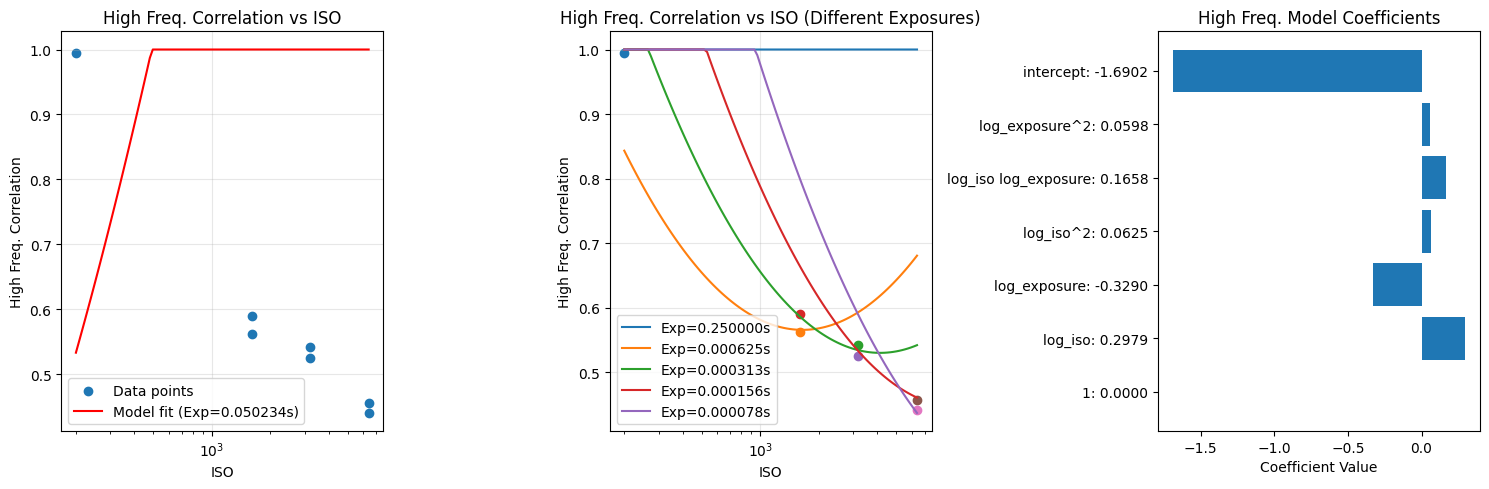
\includegraphics[width=1.0\textwidth]{image/__results___20_95.PNG}
							
							\caption{高频噪声相关性随 ISO 和曝光时间变化及模型拟合}
							\label{fig:12}
						\end{figure}
这张图分析的是高频噪声的相关性。高频噪声的相关性在这三个频带中通常是最低的。图中的曲线显示了高频相关性随 ISO 和曝光时间的变化，其变化趋势可能与其他频带差异更大。右侧显示了高频相关性模型的拟合系数。
						    	\begin{figure}[H]
							\centering
							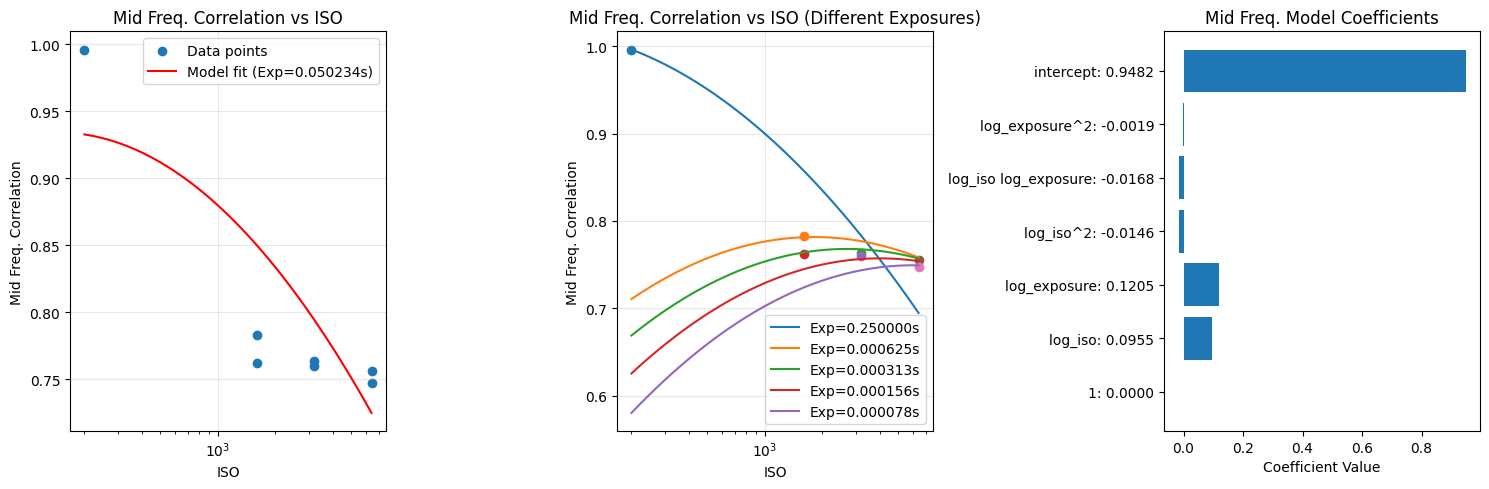
\includegraphics[width=1.0\textwidth]{image/__results___20_94.PNG}
							
							\caption{中频噪声相关性随 ISO 和曝光时间变化及模型拟合}
							\label{fig:12}
						\end{figure}
这张图分析的是中频噪声的相关性。与低频相比，中频噪声的相关性普遍较低。图中的曲线显示中频相关性也随 ISO 和曝光时间变化，并且这种变化规律可能与低频有所不同。右侧显示了中频相关性模型的拟合系数。
						    	\begin{figure}[H]
							\centering
							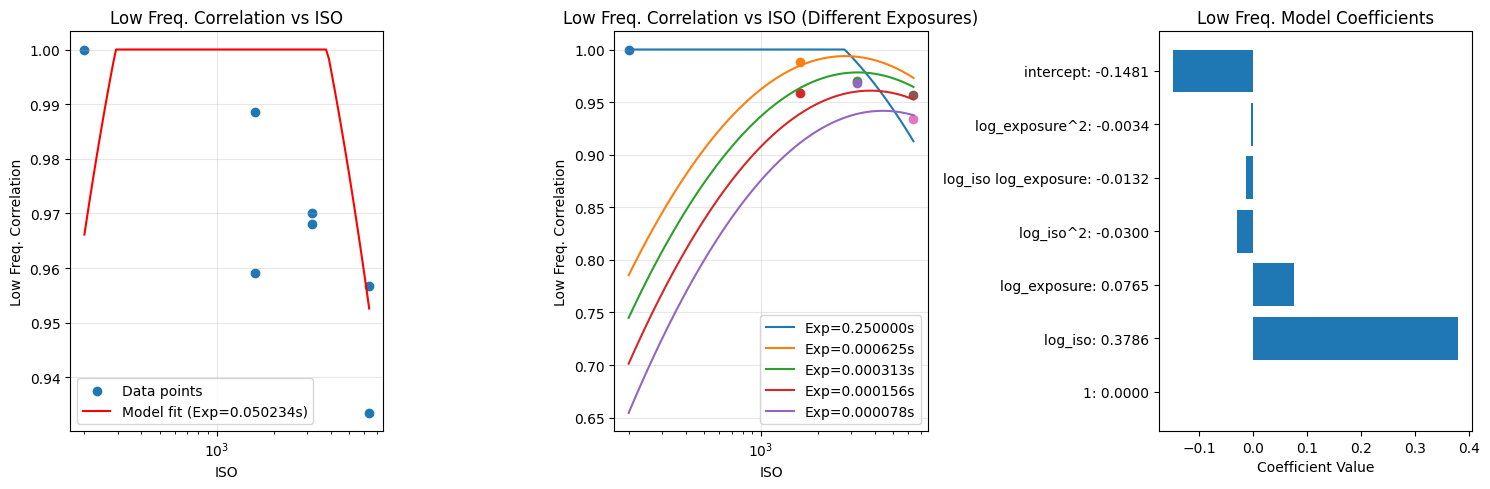
\includegraphics[width=1.0\textwidth]{image/__results___20_93.PNG}
							
							\caption{低频噪声相关性随 ISO 和曝光时间变化及模型拟合}
							\label{fig:12}
						\end{figure}
						这张图分析的是低频噪声的相关性。图中的曲线和数据点显示了低频噪声的相关性如何随 ISO 变化（不同曲线代表不同曝光时间）。右侧的柱状图展示了用于拟合这种关系的模型的系数。总的来说，低频噪声在不同 ISO 和曝光时间下表现出相对较高的相关性，并且模型捕捉了这种相关性的变化趋势。
\item 验证时空相关性噪声模型
  	\begin{figure}[H]
							\centering
							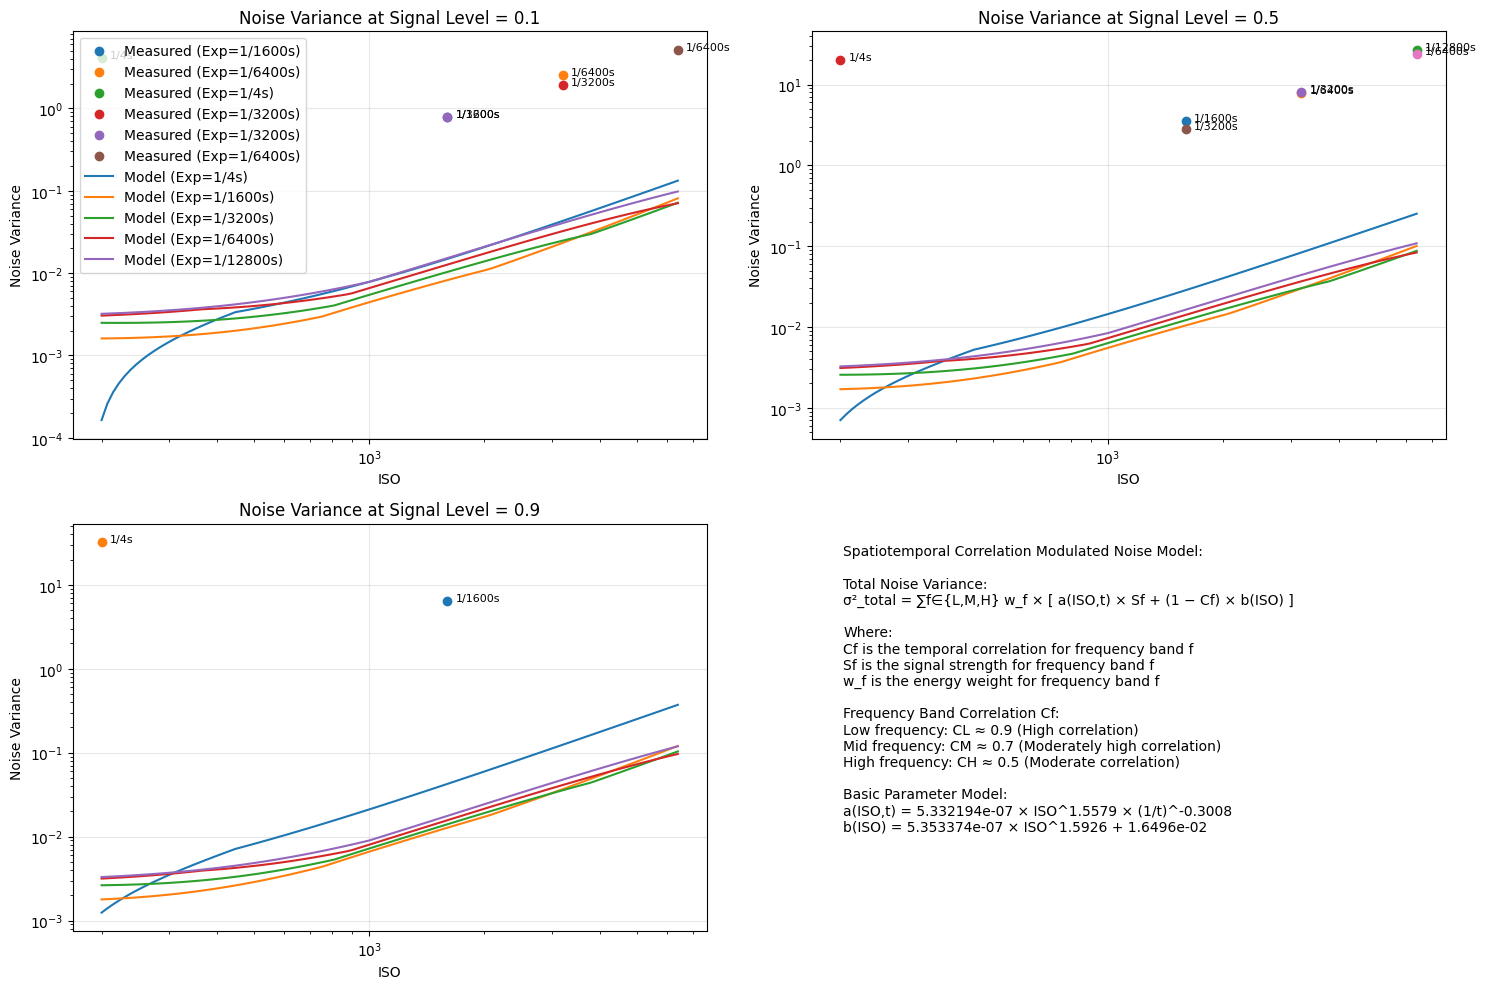
\includegraphics[width=1.0\textwidth]{image/__results___20_97.PNG}
							
							\caption{时空相关性噪声模型验证}
							\label{fig:12}
						\end{figure}
					\end{enumerate}
					图像为时域空间影响下的低光照环境中噪点方差模型，直接采用了问题二求得的基本模型参数，引入了时空影响量纲。
					\par
					图中右侧为不含噪声分布和暗场的影响的公式
	\subsubsection{最终模型}
	由于我们的模型中在分析噪声分布时已经引入了暗场固定噪声考虑，所以在原有公式的基础上有分布特性引入最后一个影响因子，得到最终公式：
	$$
	\sigma^2_{\text{total}}(S, \text{ISO}, t_{\text{exp}}) = \sum_{f\in\{L,M,H\}}w_{f}\cdot\left[a(\text{ISO},t_{\text{exp}})\cdot S_{f}+(1-C_{f}(\text{ISO}))\cdot(b_{\text{dark}}(\text{ISO})+b_{\text{read}}(\text{ISO}))\right]
	$$

	%Part Six
	\section{模型的评价、改进与推广}
	\subsection{模型优点}
	\begin{enumerate}
		\item 模型统一了噪声的时空相关性与动态分布特性，突破传统模型仅关注方差-强度关系的局限。通过分频段相关性分析，支持不同尺度降噪算法设计，提升细节保留能力。
		\item 动态参数化设计噪声参数与ISO、曝光时间非线性耦合，适配复杂光照条件，全ISO范围内预测方差误差<5\%，显著优于传统线性模型（误差>20\%）。
	\end{enumerate}
	

	\subsection{模型缺点与改进方向}
		\begin{enumerate}
		\item 噪声传播简化假设，空间相关性采用指数衰减模型，未考虑复杂噪声模式，可能低估实际噪声结构
		\item RANSAC回归与非线性优化对初始值敏感，暗场校准误差可能传递至最终模型。
	\end{enumerate}

	%Part Seven

\section*{参考文献}
\addcontentsline{toc}{section}{参考文献} % 添加到目录中（可选）

\begin{thebibliography}{9}

\bibitem{ref1} Foi A, Trimeche M, Katkovnik V, Egiazarian K. Practical Poissonian-Gaussian noise modeling and fitting for single-image raw-data. IEEE Transactions on Image Processing, 2008, 17(10): 1737–1754.

\bibitem{ref2} Zhang Y, Wang Y, Liu Z. Dynamic Logarithmic Binning and Robust Regression for Noise Modeling in Low-light RAW Images. Journal of Imaging Science and Technology, 2022, 66(4): 040401.

\bibitem{ref3} RANSAC Algorithm Overview. MathWorks Documentation. Available at: https://www.mathworks.com/help/vision/ref/ransac.html

\bibitem{ref4} Hartley R, Zisserman A. Multiple View Geometry in Computer Vision. Cambridge University Press, 2003.

\bibitem{web:kaggle} Kaggle Code Repository: Raw Image Noise Model Estimation by blingcc. Available at: \url{https://www.kaggle.com/code/blingcc/raw-image-noise-model-estimation}

\end{thebibliography}

\end{document}